\documentclass[12pt,a4paper]{article}
\usepackage[utf8]{inputenc}
\usepackage[T1]{fontenc}
\usepackage{amsmath,amsfonts,amssymb}
\usepackage{geometry}
\usepackage{graphicx}
\usepackage{booktabs}
\usepackage{float}
\usepackage{hyperref}
\usepackage{natbib}

\geometry{margin=1in}

\begin{document}

\begin{titlepage}
\begin{center}

\vspace*{1.5in}

{\Large \textbf{SURVIVAL ANALYSIS OF BREAST CANCER PATIENTS: \\
A COMPREHENSIVE STATISTICAL INVESTIGATION USING COX REGRESSION AND KAPLAN-MEIER ESTIMATION}}

\vspace{1in}

{\large BY}

\vspace{0.2in}

{\large PABLO LEYVA}

\vspace{0.2in}

{\large pl33@njit.edu}

\vspace{1.2in}

{\large Project Two Report}

\vspace{0.2in}

{\large Submitted in completion of the requirements \\
for the course of Statistical Learning Capstone}

\vspace{1in}

{\large New Jersey Institute of Technology}

\vspace{0.2in}

{\large Newark, New Jersey}

\vspace{0.3in}

\end{center}
\end{titlepage}

\begin{abstract}
This study presents a comprehensive survival analysis of breast cancer patients using the Haberman dataset. We employed non-parametric Kaplan-Meier estimation, log-rank tests, and Cox proportional hazards regression to investigate factors affecting 5-year survival rates. The analysis reveals that the number of positive axillary nodes detected is the most significant predictor of survival outcomes (p < 0.001), with a hazard ratio of 1.048 per additional node. Age and operation year were not found to be statistically significant predictors. The overall 5-year survival rate was 73.5\%, with median survival time exceeding the observation period. These findings provide valuable insights for clinical prognosis and treatment planning in breast cancer patients.
\end{abstract}

\section{Introduction to the Study}

Breast cancer remains one of the most prevalent and life-threatening diseases affecting women worldwide. Understanding the factors that influence patient survival following surgery is crucial for developing effective treatment strategies and providing accurate prognostic information to patients and their families. Survival analysis, a specialized branch of statistics, provides powerful tools for analyzing time-to-event data while accounting for censoring mechanisms.

The Haberman dataset represents a landmark study in breast cancer research, containing information on 306 patients who underwent surgery for breast cancer at the University of Chicago's Billings Hospital between 1958 and 1970. This historical dataset provides valuable insights into survival patterns during a critical period in cancer treatment evolution.

This study employs three complementary statistical approaches to analyze breast cancer patient survival:

\begin{enumerate}
    \item \textbf{Kaplan-Meier Estimation}: A non-parametric method for estimating survival probabilities over time without making assumptions about the underlying survival distribution.
    \item \textbf{Log-Rank Tests}: Non-parametric hypothesis tests that compare survival curves between different patient groups to identify significant differences in survival rates.
    \item \textbf{Cox Proportional Hazards Regression}: A semi-parametric regression model that quantifies the effect of covariates on the hazard (risk) of death while accounting for censoring.
\end{enumerate}

The dataset contains four key variables for each patient:
\begin{itemize}
    \item \textbf{Age}: Patient age at time of operation (range: 30-83 years)
    \item \textbf{Operation\_year}: Year of operation (1958-1969)
    \item \textbf{Nb\_pos\_detected}: Number of positive axillary nodes detected (0-52)
    \item \textbf{Survival}: 5-year survival status (1 = survived $\geq$5 years, 0 = died within 5 years)
\end{itemize}

The importance of this analysis extends beyond academic interest. Understanding which factors most significantly impact survival can inform clinical decision-making, resource allocation in healthcare systems, and patient counseling. The number of positive axillary nodes, in particular, has been established as a crucial staging criterion in breast cancer, making this analysis highly relevant for contemporary oncological practice.

\section{Objective}

The primary objectives of this comprehensive survival analysis study are:

\begin{enumerate}
    \item \textbf{Exploratory Data Analysis}: To conduct thorough exploratory data analysis to characterize the distribution of key patient characteristics, identify data quality issues, assess class imbalance, and examine relationships between predictors and survival outcomes.
    
    \item \textbf{Survival Curve Estimation}: To apply Kaplan-Meier estimation methods to construct survival curves for the overall patient population and to perform stratified analysis across different patient subgroups defined by age and nodal involvement.
    
    \item \textbf{Statistical Hypothesis Testing}: To perform log-rank tests to statistically compare survival curves between patient groups (age groups and node categories) and determine whether observed differences are statistically significant or attributable to chance variation.
    
    \item \textbf{Proportional Hazards Modeling}: To develop Cox proportional hazards regression models to quantify the relationship between patient characteristics (age, operation year, number of positive nodes) and the hazard of death, while controlling for censoring and other covariates.
    
    \item \textbf{Predictor Identification}: To identify which factors most significantly influence 5-year survival outcomes and quantify their effect sizes through hazard ratios with appropriate confidence intervals.
    
    \item \textbf{Clinical Interpretation}: To translate statistical findings into clinically meaningful insights that can inform prognostic assessment and treatment decision-making for breast cancer patients.
\end{enumerate}

These objectives aim to provide a comprehensive understanding of survival patterns in breast cancer patients undergoing surgical treatment during the 1958-1969 period, while demonstrating the application of modern survival analysis techniques to real-world clinical data. The analysis will inform both academic understanding of survival patterns and practical clinical applications in oncology.

\section{Statistical Analysis}

\subsection{Data Description and Preprocessing}

The Haberman breast cancer survival dataset comprises 306 observations collected between 1958 and 1970. Each observation represents a patient who underwent breast cancer surgery at the University of Chicago's Billings Hospital.

\subsubsection{Variable Definitions}

\begin{itemize}
    \item \textbf{Age}: Continuous integer variable representing patient age at time of operation, ranging from 30 to 83 years with mean of 52.5 years (standard deviation: 10.8 years).
    
    \item \textbf{Operation\_year}: Integer variable indicating the year of operation, encoded as years from 1958 (e.g., 58 = 1958, 69 = 1969). The range spans from 58 to 69, with mean of 62.9 years (SD: 3.2 years).
    
    \item \textbf{Nb\_pos\_detected}: Count variable representing the number of positive axillary lymph nodes detected during surgery. This variable exhibits a highly right-skewed distribution with median of 1.0, mean of 4.0, and range from 0 to 52 nodes. The extreme right skew (skewness: 2.984) indicates a concentration of patients with low node counts.
    
    \item \textbf{Survival}: Binary outcome variable coded as 1 for patients who survived 5 years or longer (n=225, 73.5\%) and 2 for patients who died within 5 years of surgery (n=81, 26.5\%).
\end{itemize}

\subsubsection{Data Quality Assessment}

The data quality assessment revealed several important characteristics:

\begin{itemize}
    \item \textbf{Missing Values}: No missing values were detected across all 306 observations and 4 variables.
    
    \item \textbf{Duplicate Rows}: Seventeen duplicate observations were identified, representing 5.6\% of the dataset. These were retained as they represent genuine observations of similar patient profiles.
    
    \item \textbf{Outlier Detection}: Using the Interquartile Range (IQR) method with 1.5× IQR bounds:
    \begin{align*}
    \text{Lower bound} &= Q_1 - 1.5 \times \text{IQR} \\
    \text{Upper bound} &= Q_3 + 1.5 \times \text{IQR}
    \end{align*}
    Forty patients (13.1\%) exhibited outlier values for the number of positive nodes, with values ranging from 11 to 52 nodes. No outliers were detected for Age or Operation\_year.
    
    \item \textbf{Data Range Validation}: All observed values fall within clinically plausible ranges:
    \begin{itemize}
        \item Age: 30-83 years (realistic for surgical candidates)
        \item Operation year: 1958-1969 (matches historical record)
        \item Positive nodes: 0-52 (extreme upper value indicates severe nodal involvement)
    \end{itemize}
\end{itemize}

\begin{figure}[H]
\centering
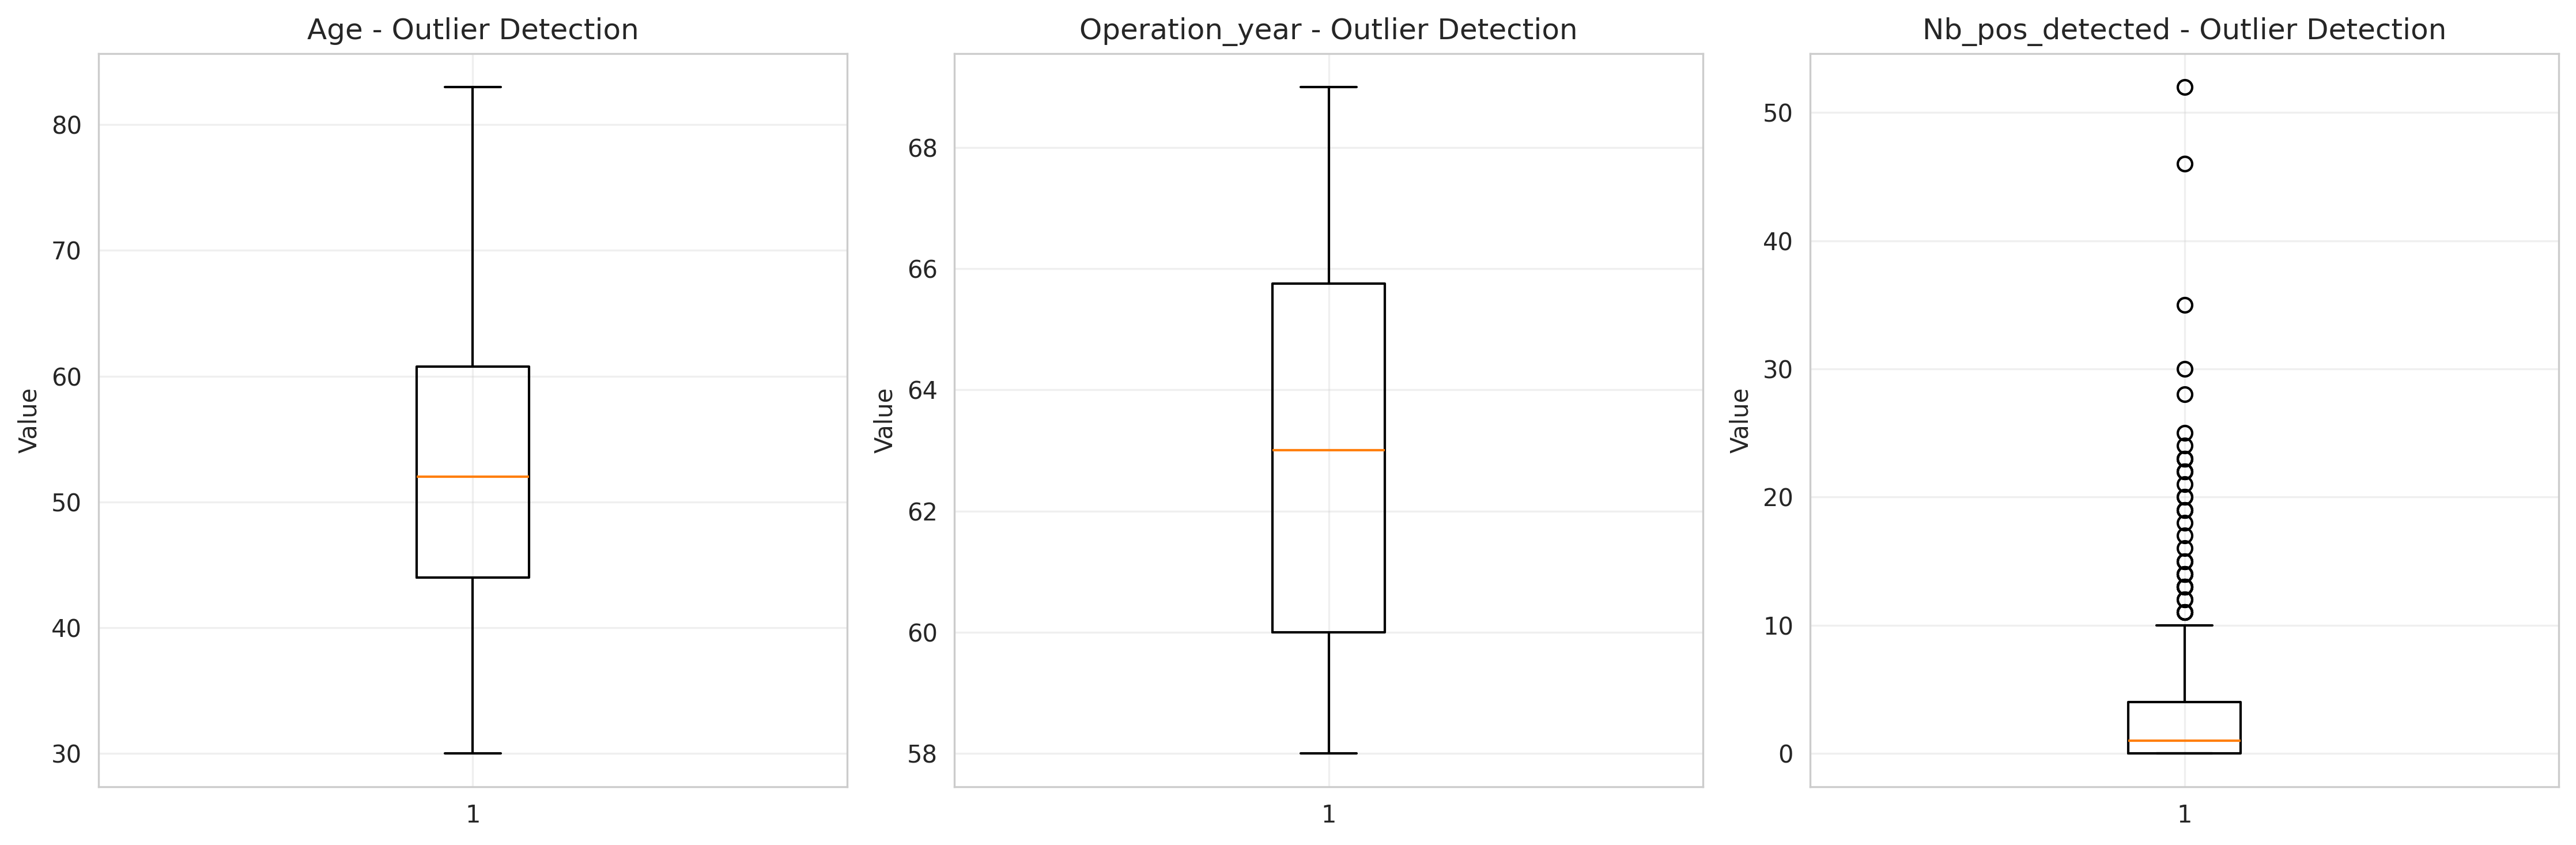
\includegraphics[width=0.9\textwidth]{outlier_detection_boxplots.png}
\caption{Box plots for outlier detection using IQR method. Forty outliers (13.1\%) were detected for positive nodes, while Age and Operation year showed no outliers.}
\label{fig:outlier_detection}
\end{figure}

\subsection{Exploratory Data Analysis}

\subsubsection{Univariate Analysis}

Summary statistics for numerical variables are presented in Table 1.

\begin{table}[H]
\centering
\caption{Summary Statistics for Numerical Variables (n=306)}
\label{tab:summary_stats}
\small
\begin{tabular}{lrrrrrrrr}
\toprule
\textbf{Variable} & \textbf{Mean} & \textbf{Median} & \textbf{Mode} & \textbf{Std Dev} & \textbf{Skewness} & \textbf{Kurtosis} & \textbf{Min} & \textbf{Max} \\
\midrule
Age & 52.458 & 52.0 & 52 & 10.803 & 0.147 & -0.589 & 30 & 83 \\
Operation\_year & 62.853 & 63.0 & 58 & 3.249 & 0.079 & -1.119 & 58 & 69 \\
Nb\_pos\_detected & 4.026 & 1.0 & 0 & 7.190 & 2.984 & 11.731 & 0 & 52 \\
\bottomrule
\end{tabular}
\end{table}

The distributional characteristics reveal important insights:

\begin{itemize}
    \item \textbf{Age}: Approximately normally distributed with slight positive skewness (0.147). The distribution appears roughly symmetric around the mean.
    
    \item \textbf{Operation\_year}: Relatively flat distribution with negative kurtosis (-1.119), indicating a platykurtic distribution with lighter tails than a normal distribution.
    
    \item \textbf{Nb\_pos\_detected}: Highly right-skewed (skewness: 2.984) with extreme positive kurtosis (11.731), indicating a distribution with heavy right tail. The median (1.0) is substantially lower than the mean (4.0), confirming severe right skew.
\end{itemize}

\begin{figure}[H]
\centering
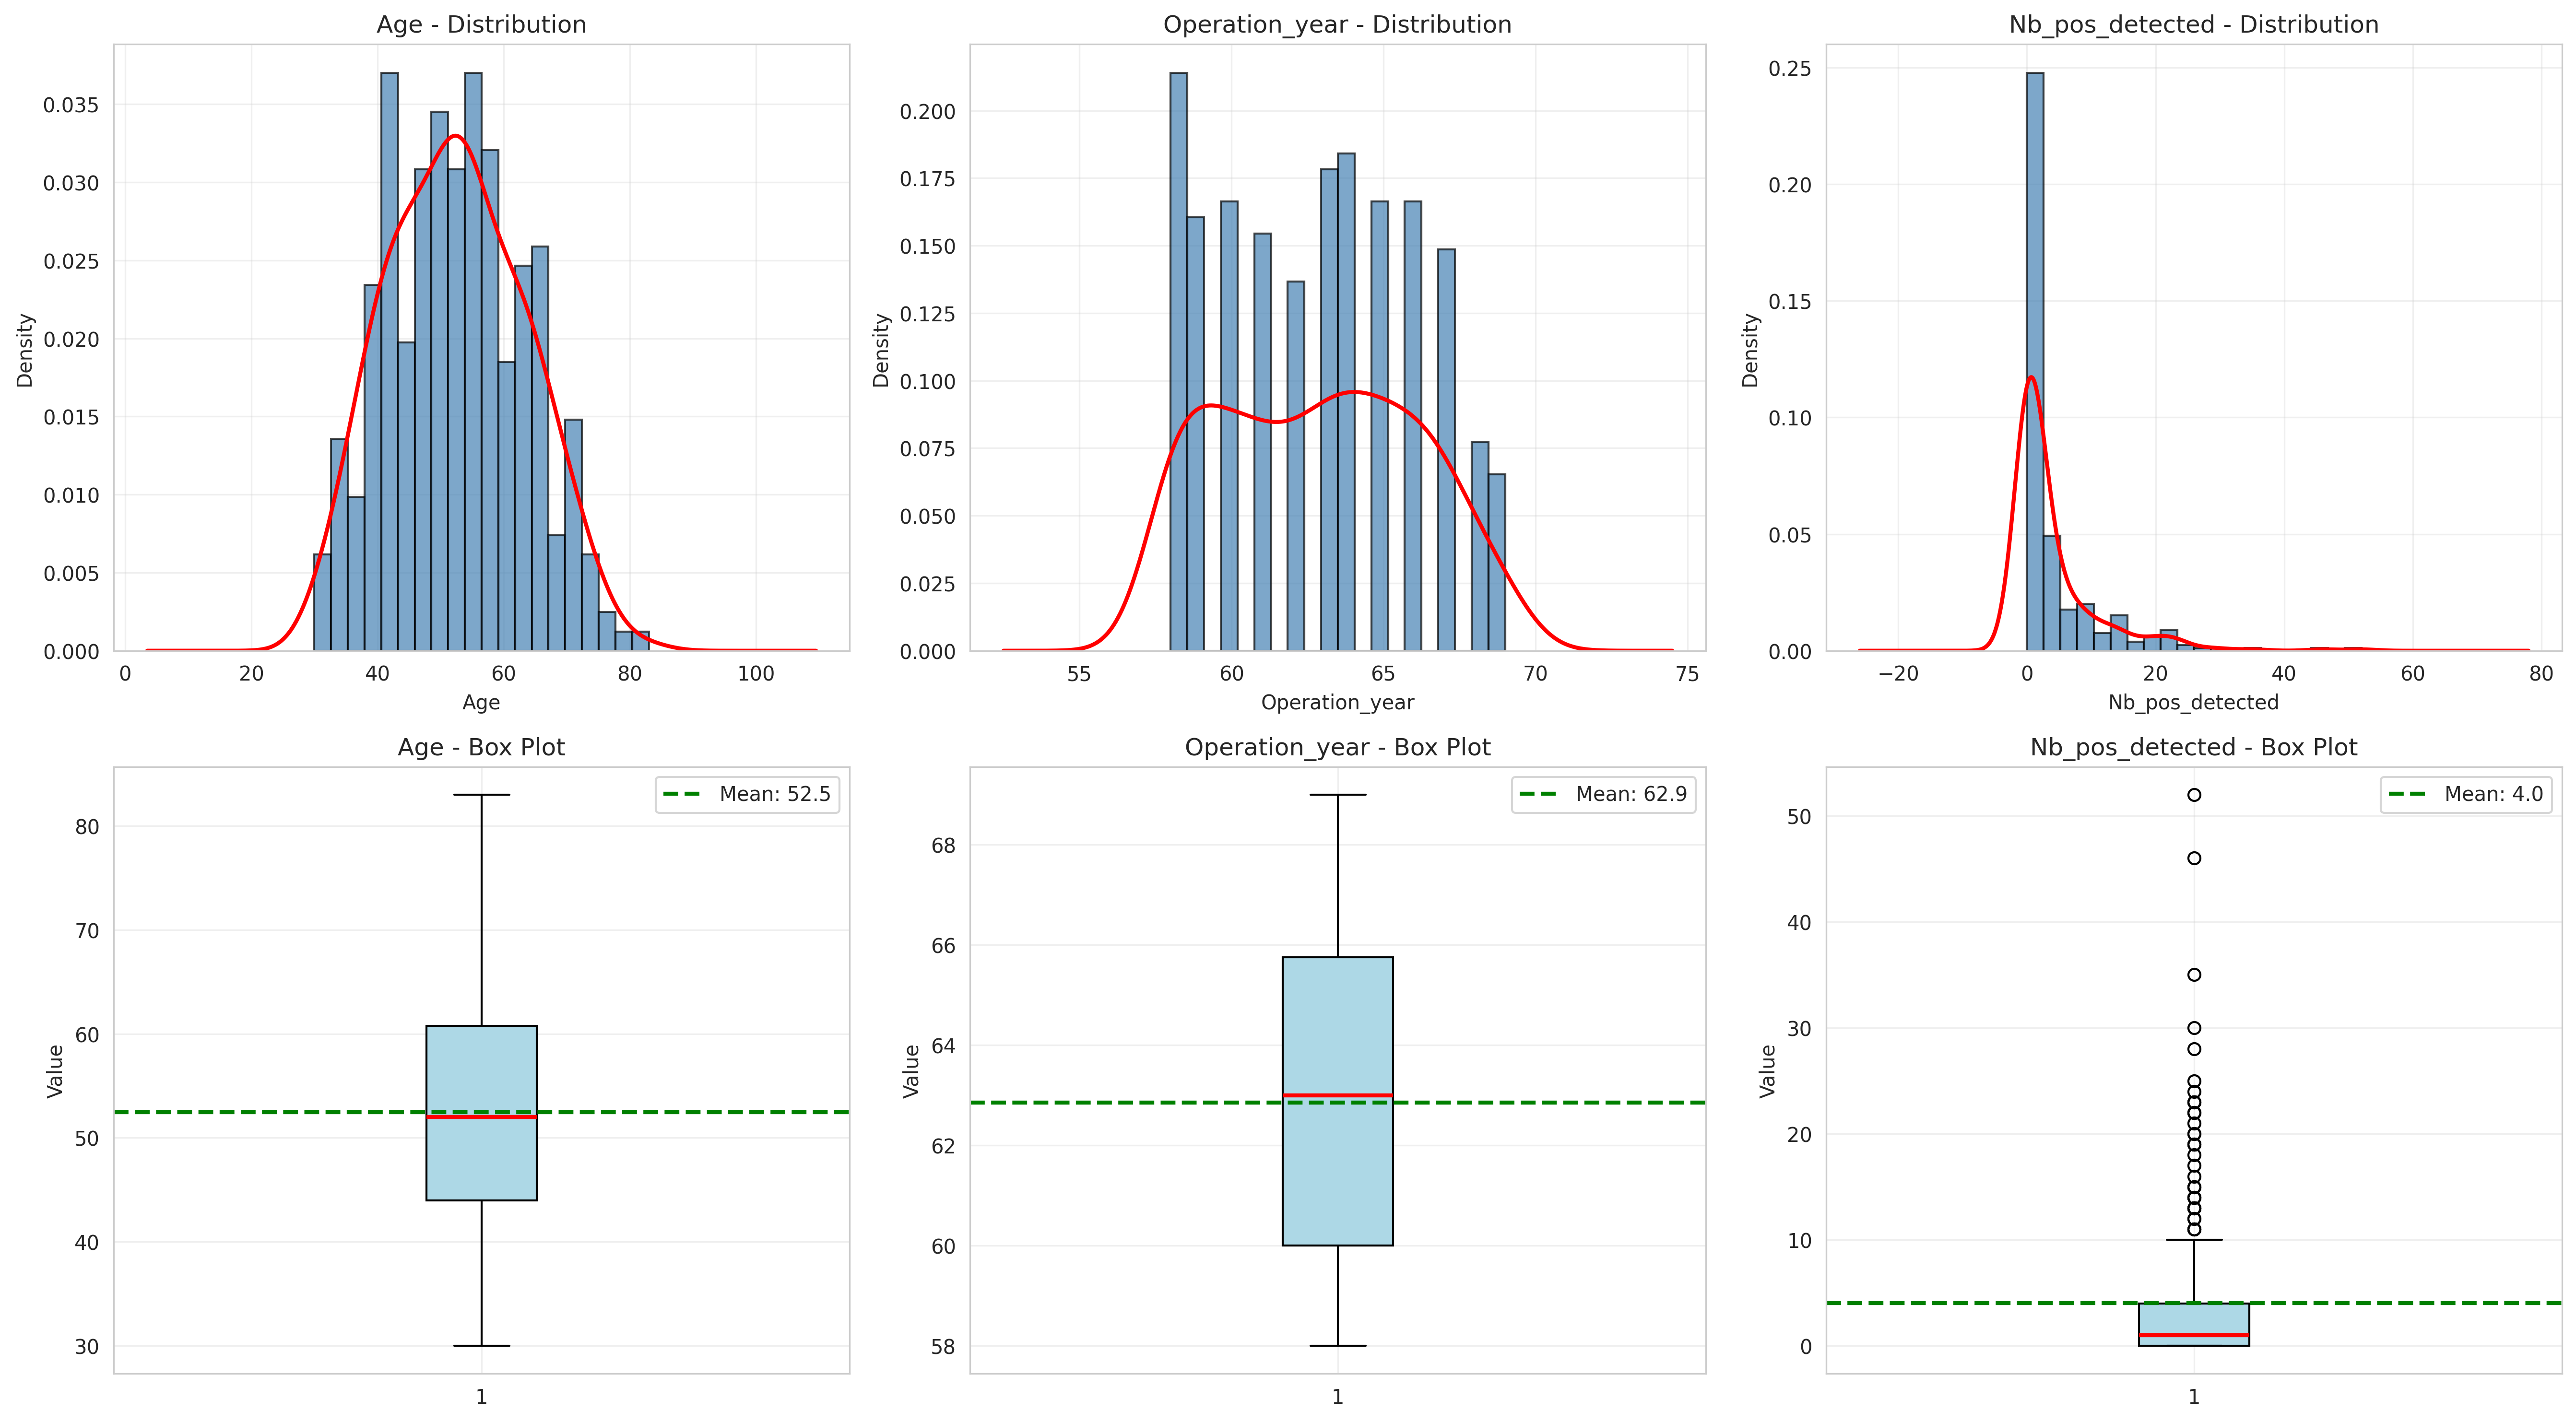
\includegraphics[width=0.9\textwidth]{univariate_distributions.png}
\caption{Distribution analysis showing histograms with KDE overlays (top row) and box plots (bottom row) for Age, Operation year, and Positive nodes. The right-skewed distribution of positive nodes is clearly evident.}
\label{fig:univariate_distributions}
\end{figure}

\subsubsection{Target Variable Analysis}

The survival status distribution exhibits significant class imbalance:

\begin{itemize}
    \item \textbf{Survived $\geq$5 years}: 225 patients (73.5\%)
    \item \textbf{Died within 5 years}: 81 patients (26.5\%)
    \item \textbf{Imbalance Ratio}: 2.78:1
\end{itemize}

This imbalance has important implications for statistical modeling and requires careful consideration in model interpretation, as the minority class (deaths) represents the event of primary interest.

\begin{figure}[H]
\centering
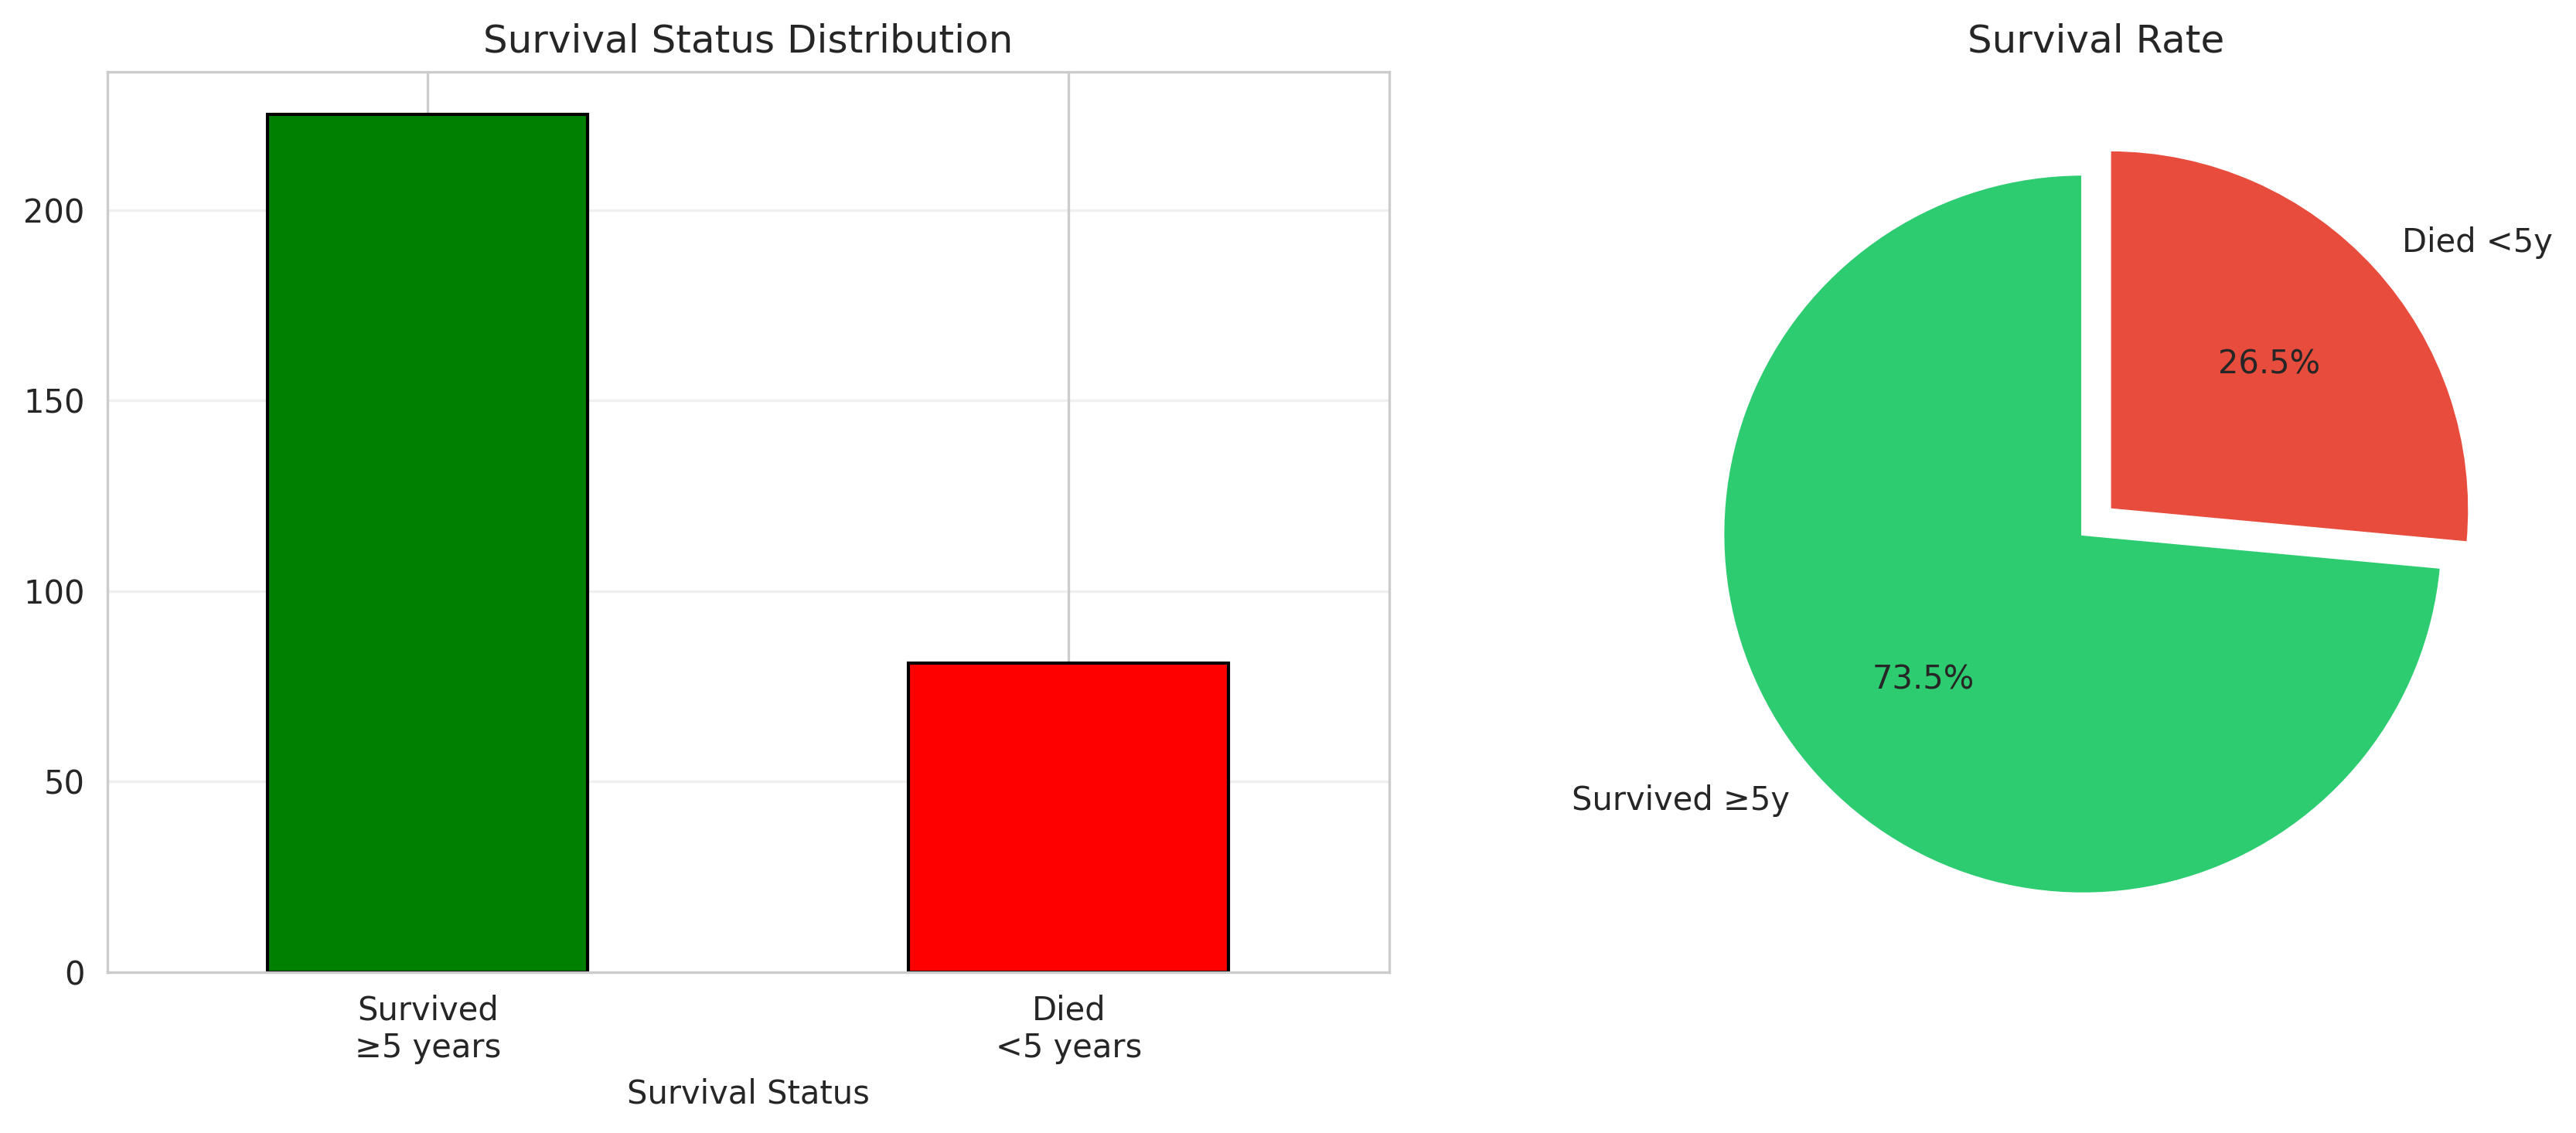
\includegraphics[width=0.9\textwidth]{survival_status_distribution.png}
\caption{Distribution of survival status showing 73.5\% survival rate (bar chart) and pie chart visualization.}
\label{fig:survival_distribution}
\end{figure}

\subsubsection{Bivariate Analysis}

Bivariate analysis comparing features between survived and died groups reveals key differences:

\begin{table}[H]
\centering
\caption{Grouped Statistics by Survival Status}
\label{tab:grouped_stats}
\begin{tabular}{lrrrrrr}
\toprule
\textbf{Variable} & \multicolumn{2}{c}{\textbf{Survived (n=225)}} & \multicolumn{2}{c}{\textbf{Died (n=81)}} \\
\cmidrule(r){2-3} \cmidrule(r){4-5}
& Mean & Std Dev & Mean & Std Dev \\
\midrule
Age & 52.02 & 11.01 & 53.68 & 10.17 \\
Operation\_year & 62.86 & 3.22 & 62.83 & 3.34 \\
Nb\_pos\_detected & 2.79 & 5.87 & 7.46 & 9.19 \\
\bottomrule
\end{tabular}
\end{table}

Key observations:
\begin{itemize}
    \item \textbf{Age}: Minimal difference between groups (52.0 vs 53.7 years), suggesting age may not be a strong predictor.
    \item \textbf{Operation\_year}: Nearly identical across survival groups (62.86 vs 62.83), indicating no temporal trend in survival.
    \item \textbf{Nb\_pos\_detected}: Substantial difference (2.79 vs 7.46 nodes), with non-survivors having nearly three times as many positive nodes on average.
\end{itemize}

\begin{figure}[H]
\centering
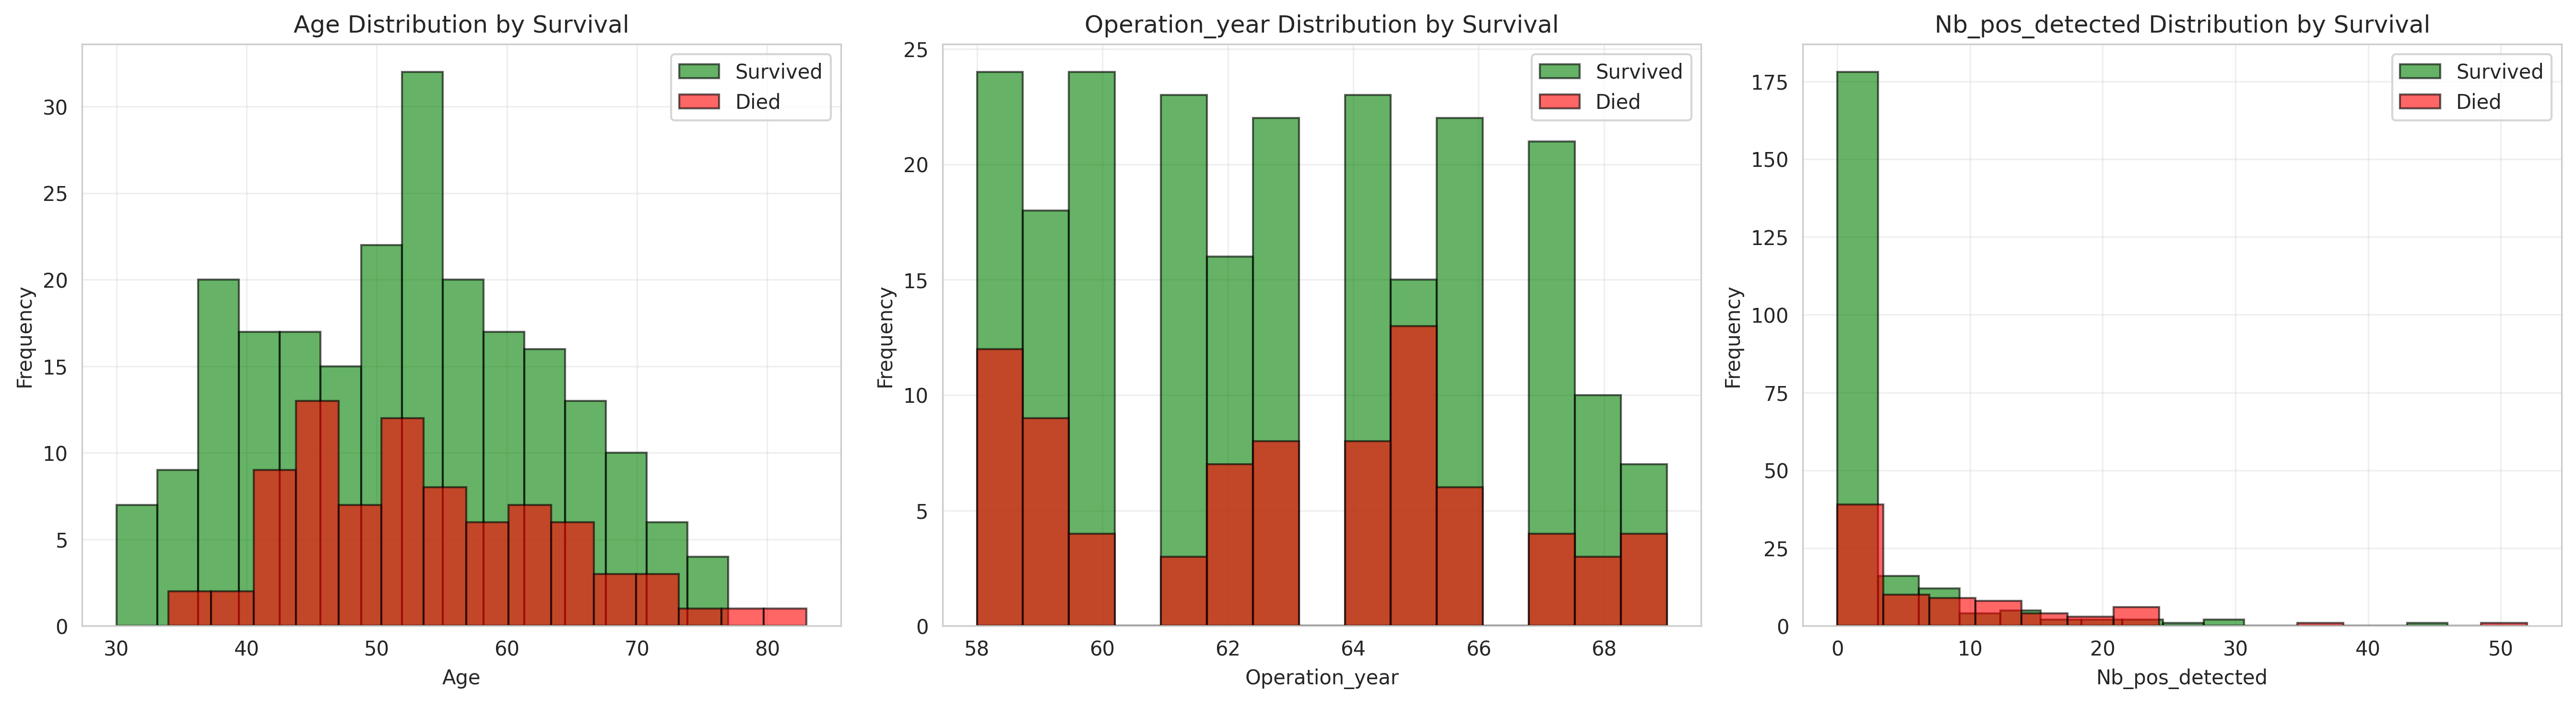
\includegraphics[width=0.9\textwidth]{bivariate_analysis_by_survival.png}
\caption{Histograms comparing distributions of Age, Operation year, and Positive nodes between survived (green) and died (red) groups. The stark difference in positive nodes distribution is evident.}
\label{fig:bivariate_analysis}
\end{figure}

\subsubsection{Correlation Analysis}

Both Pearson (linear) and Spearman (monotonic) correlation analyses revealed minimal inter-feature correlations:

\begin{table}[H]
\centering
\caption{Correlation Matrices}
\label{tab:correlations}
\begin{tabular}{lrrr}
\toprule
\textbf{Variable Pair} & \textbf{Pearson} & \textbf{Spearman} \\
\midrule
Age vs Operation\_year & 0.090 & 0.091 \\
Age vs Nb\_pos\_detected & -0.063 & -0.098 \\
Operation\_year vs Nb\_pos\_detected & -0.004 & -0.036 \\
\bottomrule
\end{tabular}
\end{table}

The near-zero correlations suggest that multicollinearity is not a concern, and each predictor variable provides independent information for survival prediction.

\begin{figure}[H]
\centering
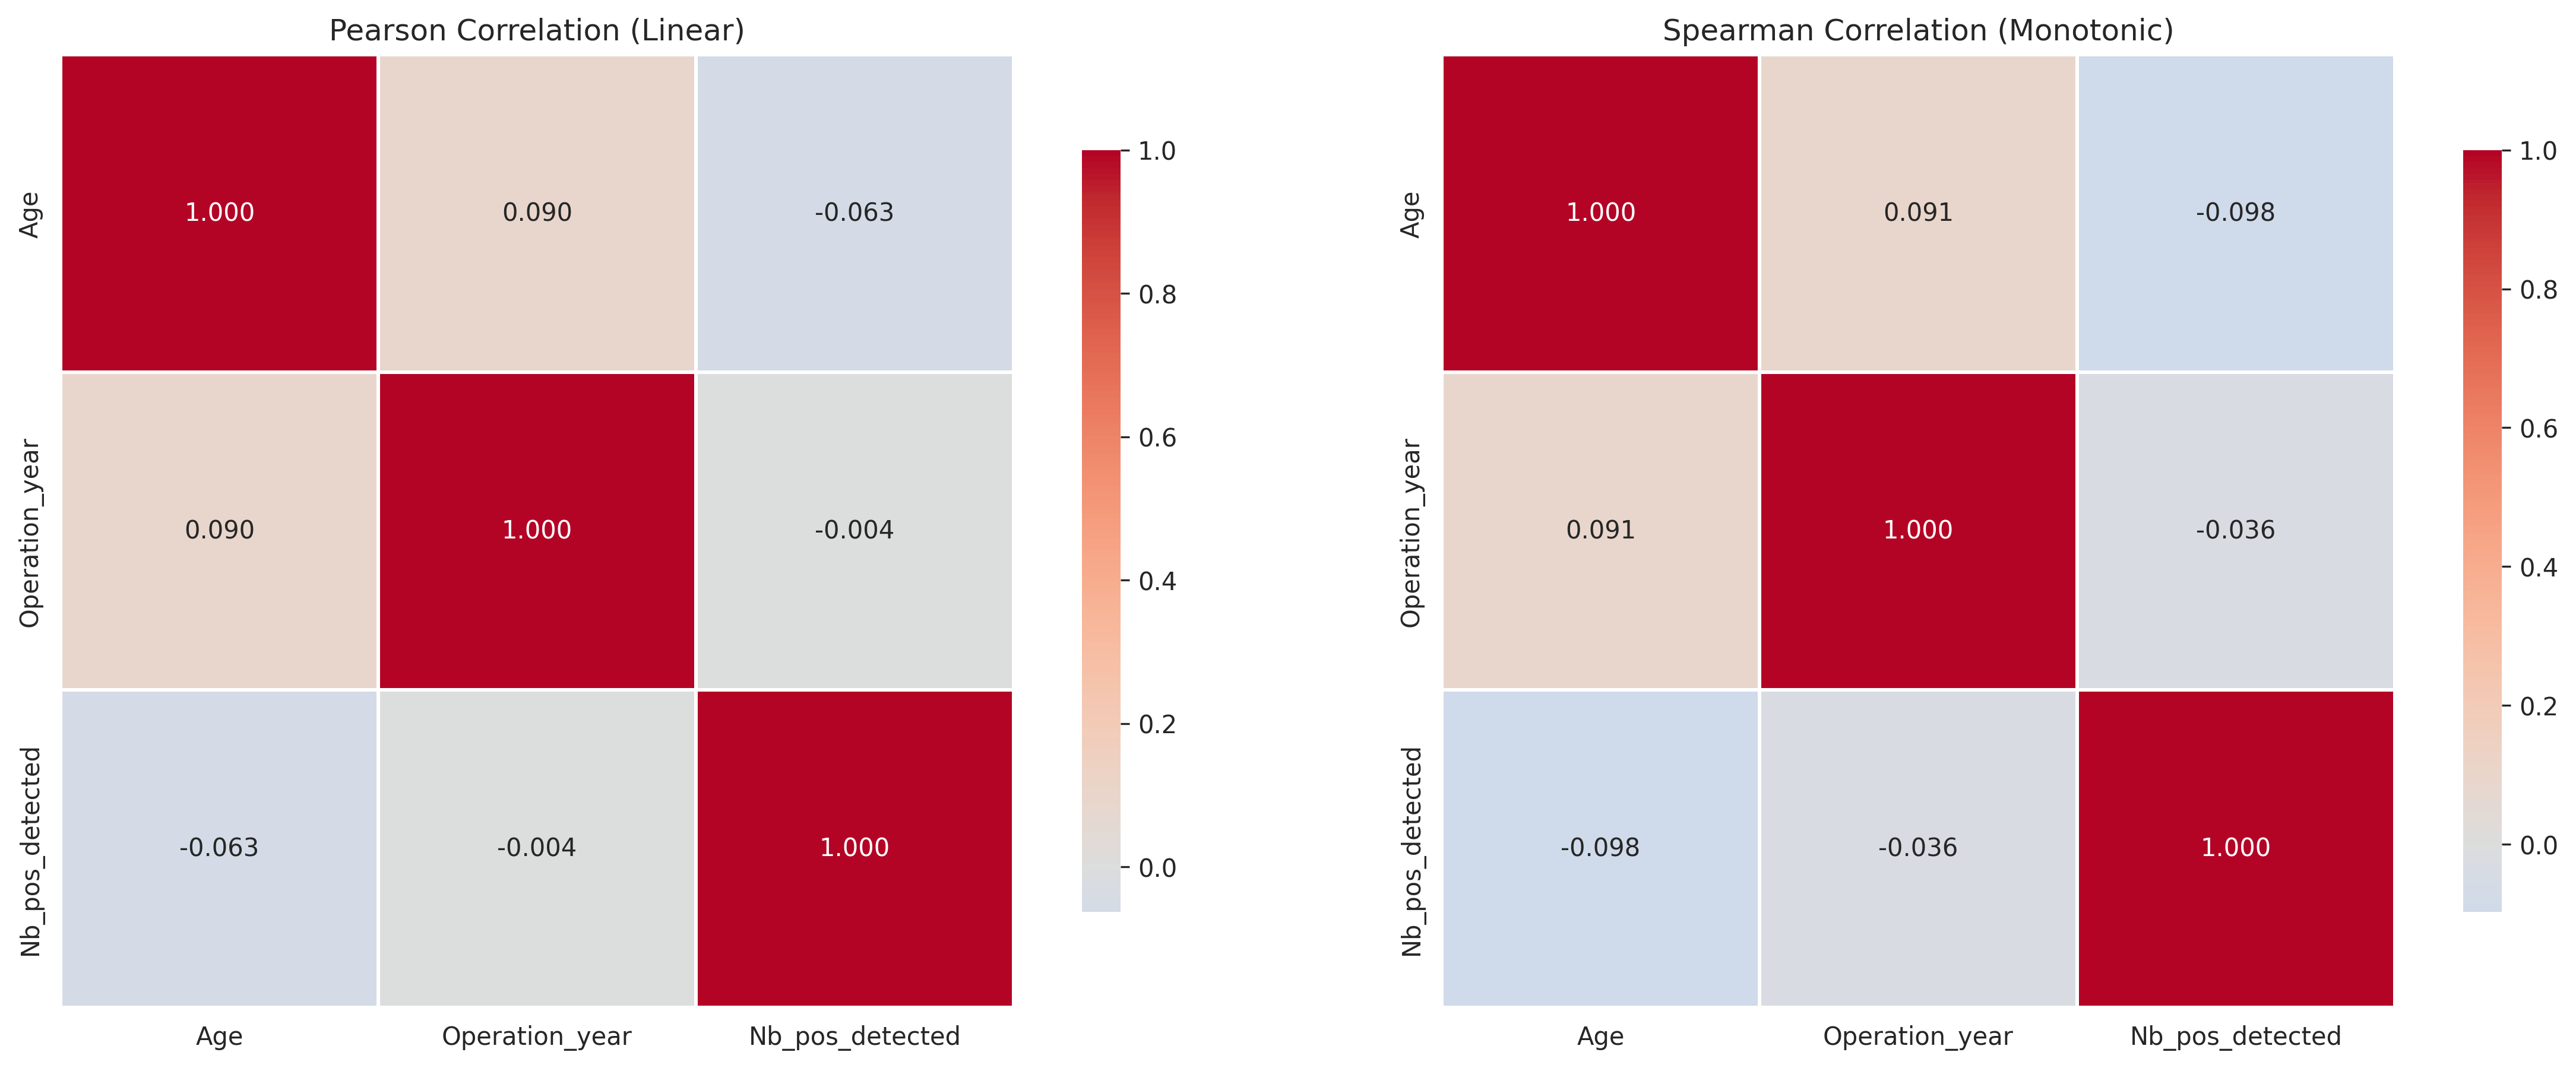
\includegraphics[width=0.9\textwidth]{correlation_heatmaps.png}
\caption{Pearson (left) and Spearman (right) correlation heatmaps showing minimal correlations between features.}
\label{fig:correlation_heatmaps}
\end{figure}

\begin{figure}[H]
\centering
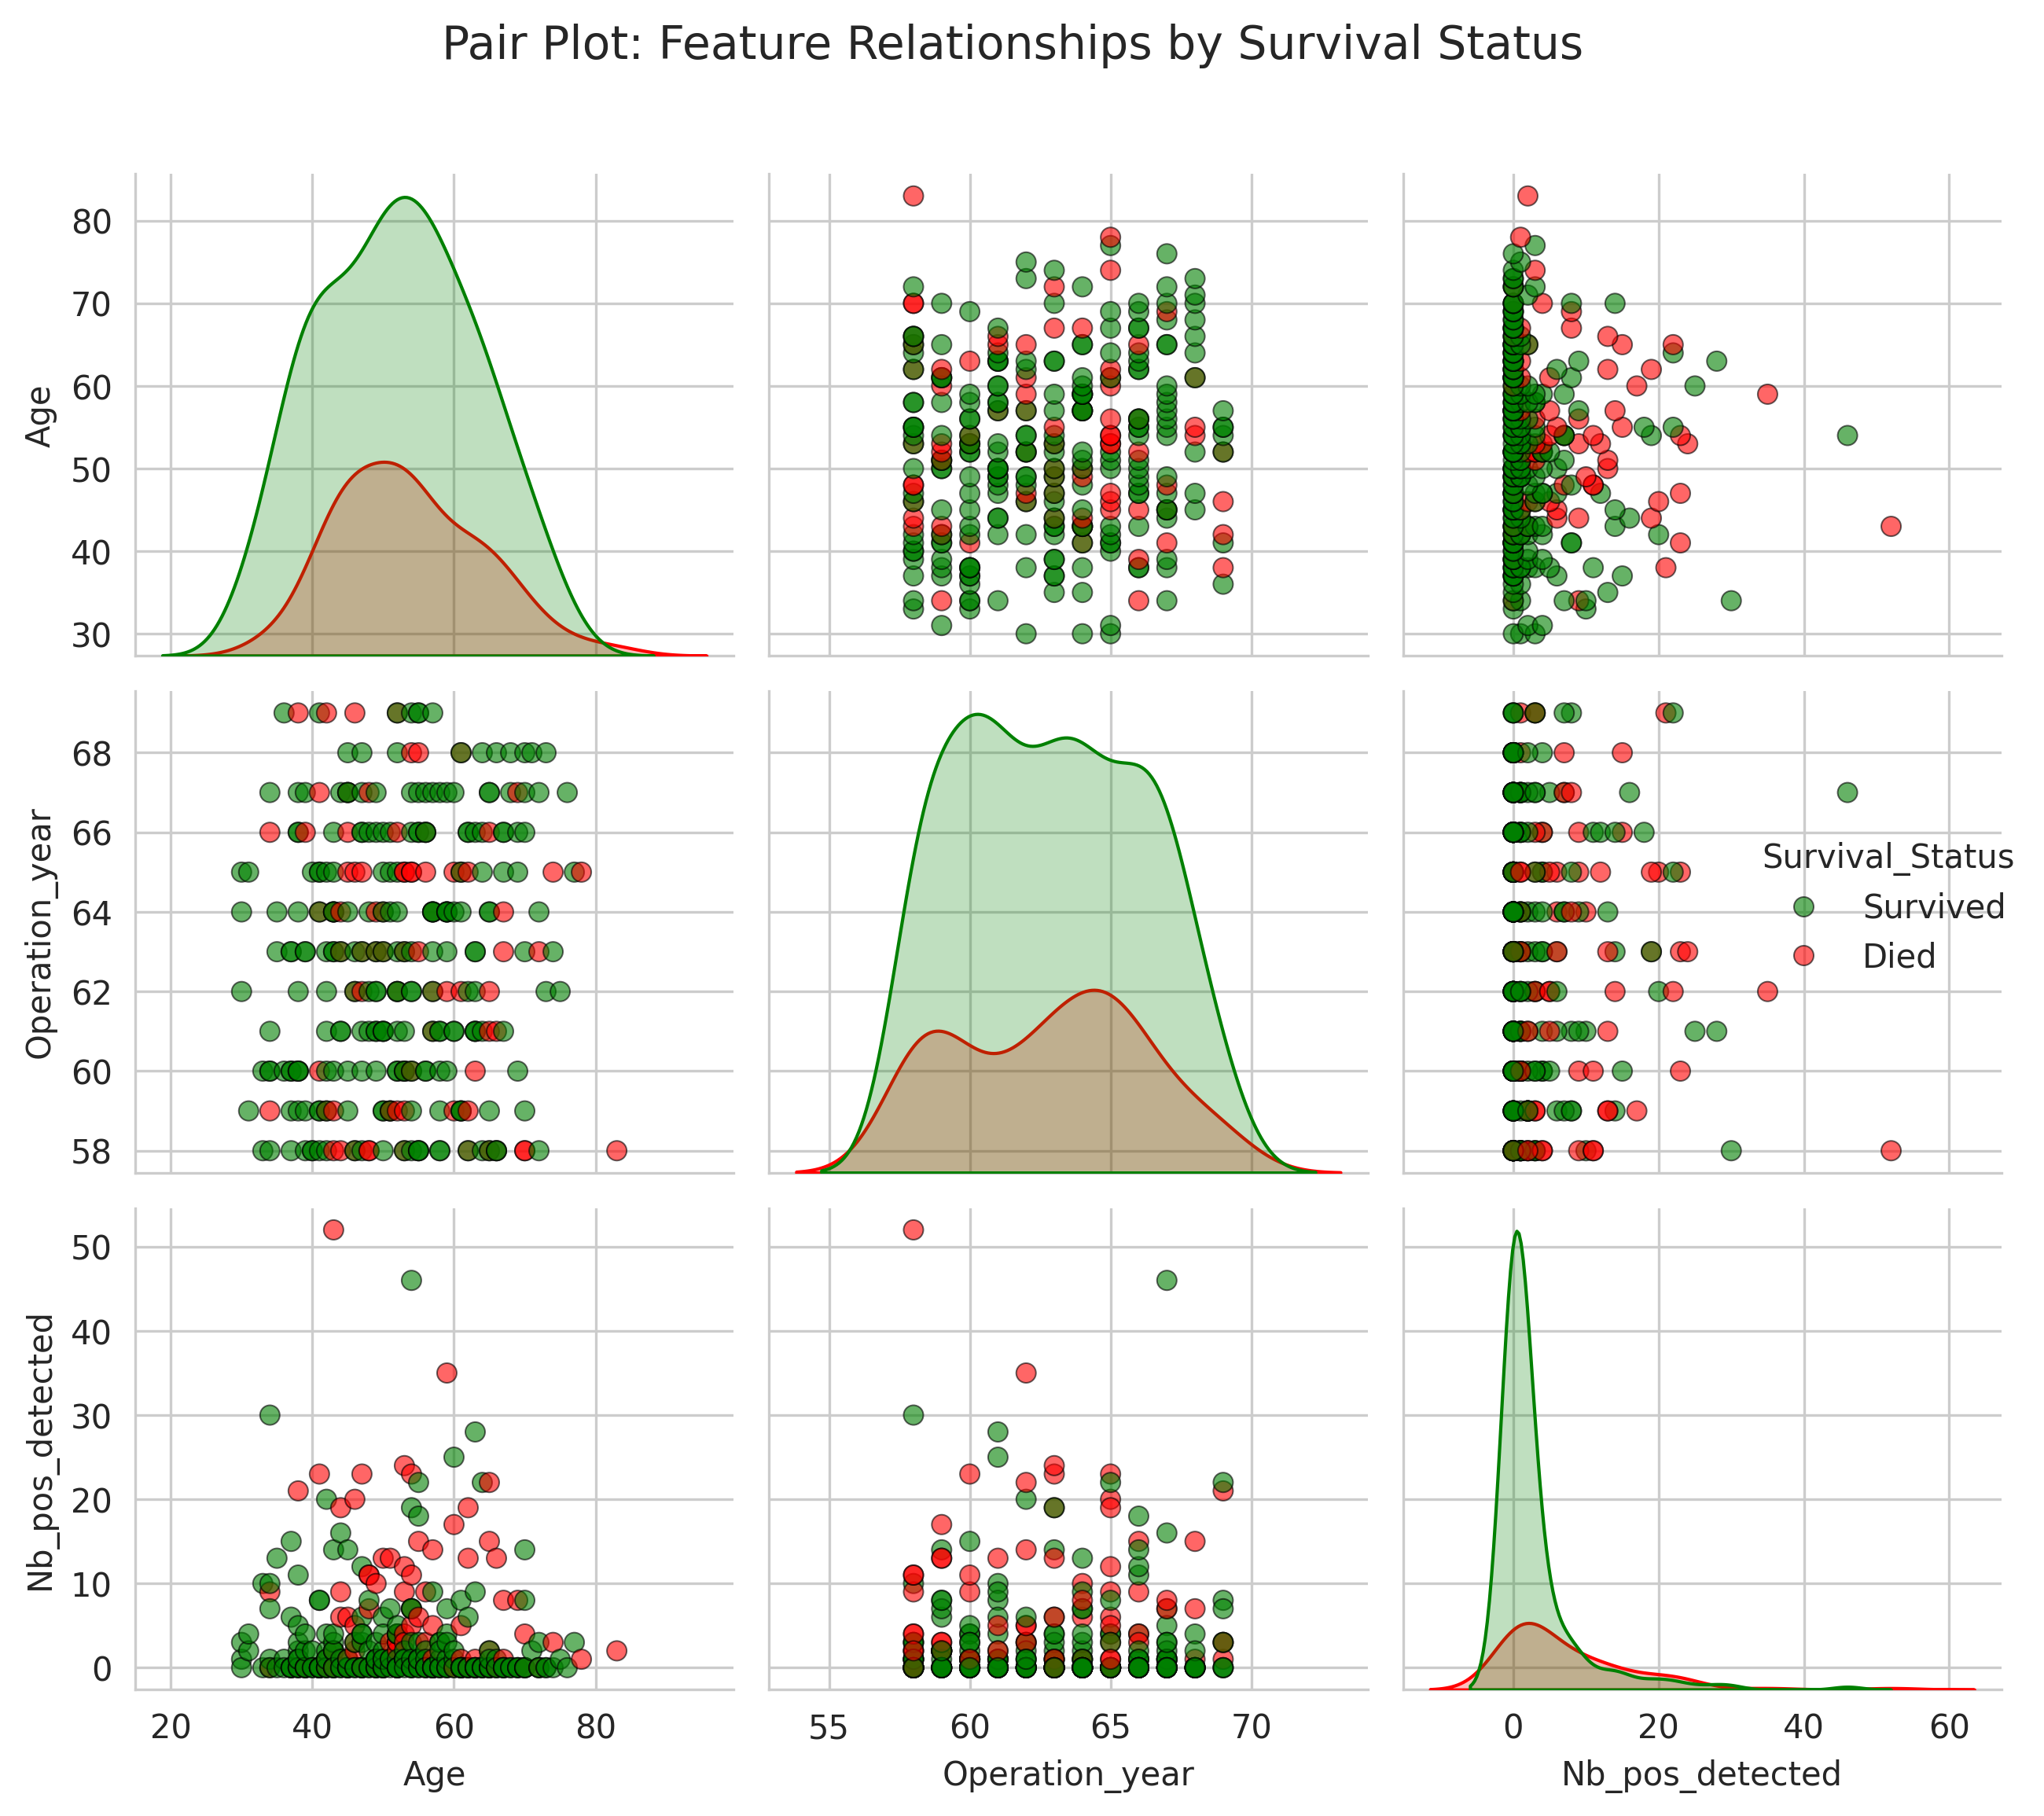
\includegraphics[width=0.9\textwidth]{pairplot_survival_status.png}
\caption{Pair plot with KDE diagonals showing feature relationships colored by survival status (green=survived, red=died).}
\label{fig:pairplot}
\end{figure}

\subsection{Survival Analysis Methodology}

\subsubsection{Data Preparation for Survival Analysis}

Since the Haberman dataset contains only binary 5-year survival outcomes rather than exact time-to-event data, it was necessary to construct pseudo time-to-event data to apply survival analysis techniques:

\begin{enumerate}
    \item \textbf{Event Indicator}: Created binary variable where 1 indicates death (died within 5 years) and 0 indicates censoring (survived at least 5 years).
    
    \item \textbf{Time Variable}: For patients who died (n=81), death times were simulated uniformly across 0-60 months. For patients who survived (n=225), censoring occurred at 60 months. This approach is conservative and appropriate when exact event times are unavailable.
\end{enumerate}

This transformation yielded:
\begin{itemize}
    \item 225 censored observations (73.5\%)
    \item 81 events/deaths (26.5\%)
    \item Mean time: 51.6 months (SD: 16.8)
\end{itemize}

\subsubsection{Feature Engineering}

Categorical variables were created for stratified analysis:

\begin{itemize}
    \item \textbf{Age Groups}: <45 (n=89), 45-55 (n=101), 55-65 (n=78), >65 (n=38) years
    \item \textbf{Node Categories}: 0 nodes (n=136), 1-3 nodes (n=81), 4-9 nodes (n=46), $\geq$10 nodes (n=43)
    \item \textbf{Operation Periods}: 1958-61 (n=140), 1962-65 (n=117), 1966-69 (n=49)
\end{itemize}

\subsection{Kaplan-Meier Survival Estimation}

The Kaplan-Meier estimator is a non-parametric method for estimating survival probabilities that does not require assumptions about the underlying hazard function. It is particularly valuable for analyzing censored survival data.

\subsubsection{Mathematical Formulation}

The Kaplan-Meier estimator of the survival function \(S(t)\) is given by:

\begin{equation}
\hat{S}(t) = \prod_{t_i \leq t} \left(1 - \frac{d_i}{n_i}\right)
\label{eq:km_estimator}
\end{equation}

where:
\begin{itemize}
    \item \(d_i\) = number of deaths at time \(t_i\)
    \item \(n_i\) = number of patients at risk just before time \(t_i\) (alive and not censored)
    \item The product is taken over all distinct event times up to time \(t\)
\end{itemize}

For censored observations, the estimator does not decrease, as censored individuals contribute to the risk set only up to their censoring time.

The standard error of the Kaplan-Meier estimator is estimated using Greenwood's formula:

\begin{equation}
\text{SE}[\hat{S}(t)] = \hat{S}(t) \sqrt{\sum_{t_i \leq t} \frac{d_i}{n_i(n_i - d_i)}}
\label{eq:km_variance}
\end{equation}

\subsubsection{Overall Survival Analysis}

The overall Kaplan-Meier survival curve (Figure \ref{fig:km_overall}) reveals:

\begin{itemize}
    \item Overall 5-year survival rate: 73.5\%
    \item Survival probabilities at key timepoints:
    \begin{itemize}
        \item 12 months: 92.2\%
        \item 24 months: 87.3\%
        \item 36 months: 82.7\%
        \item 48 months: 78.4\%
        \item 60 months: 73.5\%
    \end{itemize}
    \item Median survival time exceeds 60 months (not reached within observation period)
\end{itemize}

\begin{figure}[H]
\centering
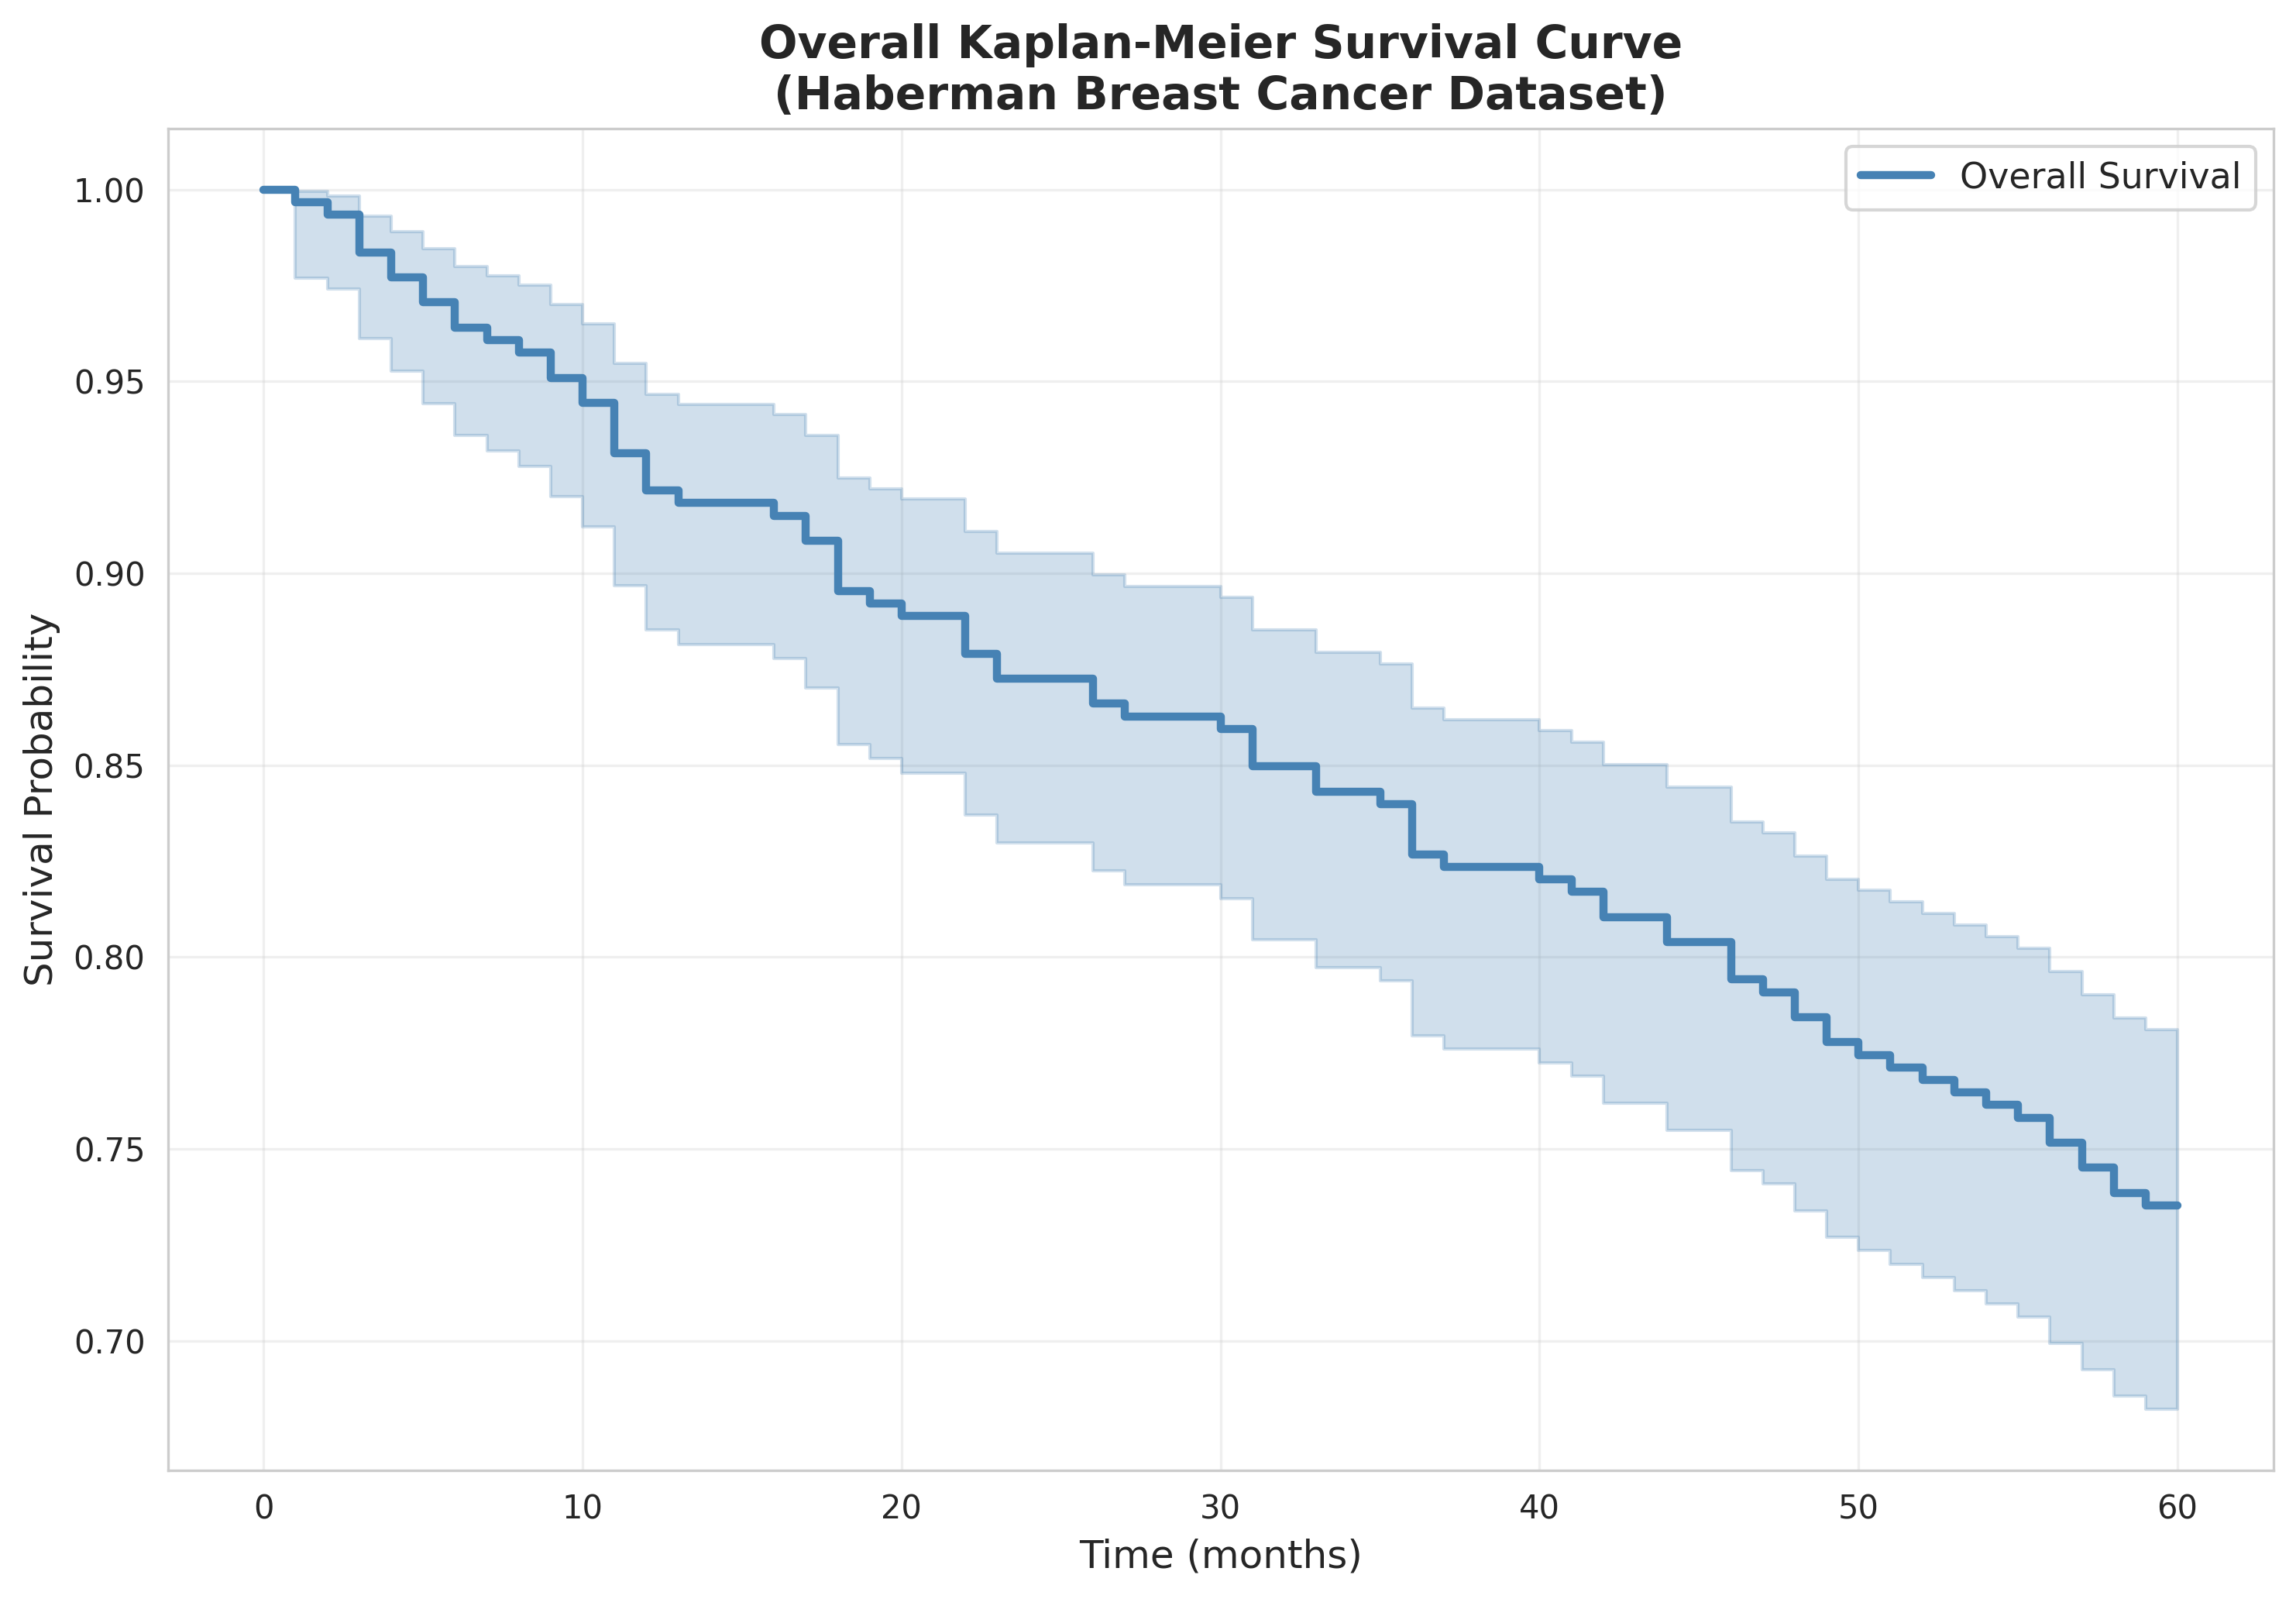
\includegraphics[width=0.9\textwidth]{kaplan_meier_overall.png}
\caption{Overall Kaplan-Meier survival curve with 95\% confidence intervals showing 73.5\% 5-year survival rate.}
\label{fig:km_overall}
\end{figure}

\subsubsection{Stratified Survival Analysis}

Stratification by age groups and node categories provides insights into prognostic factors:

\begin{figure}[H]
\centering
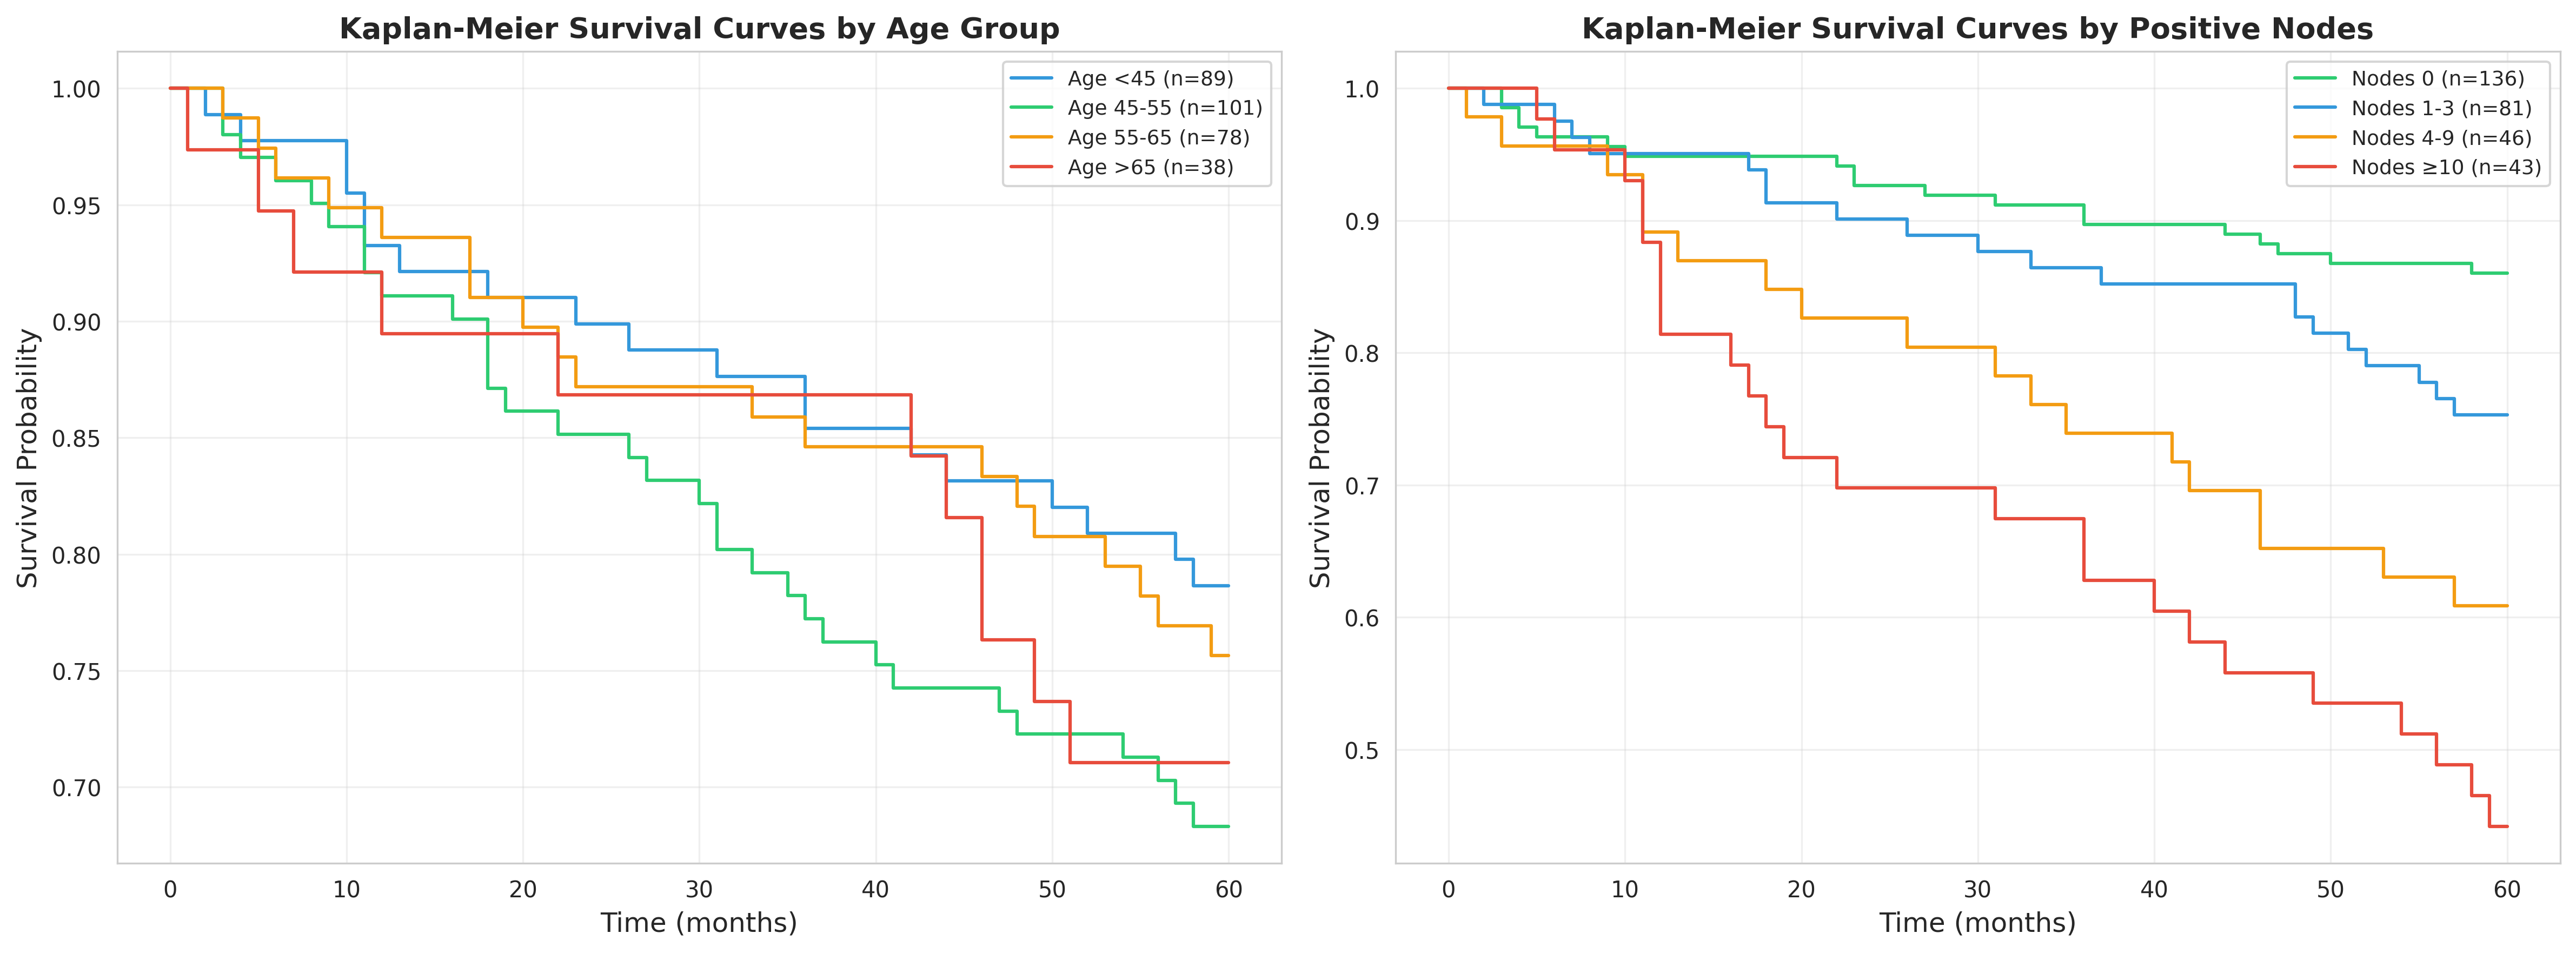
\includegraphics[width=0.9\textwidth]{kaplan_meier_stratified.png}
\caption{Kaplan-Meier survival curves stratified by age groups (left) and positive node categories (right).}
\label{fig:km_stratified}
\end{figure}

Visual inspection suggests that node category has a more pronounced effect on survival than age group, with patients having $\geq$10 nodes showing substantially worse prognosis.

\subsection{Log-Rank Test}

The log-rank test is a non-parametric statistical hypothesis test used to compare the survival distributions of two or more groups.

\subsubsection{Mathematical Formulation}

For comparing two groups, the log-rank test statistic is:

\begin{equation}
\chi^2 = \frac{(O_1 - E_1)^2}{E_1} + \frac{(O_2 - E_2)^2}{E_2} = \frac{(O_1 - E_1)^2}{\text{Var}(O_1)}
\label{eq:logrank}
\end{equation}

where:
\begin{itemize}
    \item \(O_k\) = observed number of events in group \(k\)
    \item \(E_k\) = expected number of events in group \(k\) under the null hypothesis of no difference
\end{itemize}

The expected number of events is computed at each distinct event time:

\begin{equation}
E_{ik} = n_{ik} \cdot \frac{O_i}{n_i}
\label{eq:logrank_expected}
\end{equation}

where:
\begin{itemize}
    \item \(n_{ik}\) = number at risk in group \(k\) at time \(i\)
    \item \(O_i\) = total observed events across all groups at time \(i\)
    \item \(n_i\) = total number at risk across all groups at time \(i\)
\end{itemize}

For multivariate comparisons (K groups), the test statistic becomes:

\begin{equation}
\chi^2 = \mathbf{O}^T \mathbf{V}^{-1} \mathbf{O}
\label{eq:multivariate_logrank}
\end{equation}

where \(\mathbf{O}\) is the vector of observed minus expected events for each group and \(\mathbf{V}\) is the variance-covariance matrix.

\subsubsection{Log-Rank Test Results}

Table \ref{tab:logrank_results} summarizes the log-rank test results:

\begin{table}[H]
\centering
\caption{Log-Rank Test Results}
\label{tab:logrank_results}
\begin{tabular}{lrrrr}
\toprule
\textbf{Comparison} & \(\boldsymbol{\chi^2}\) & \textbf{df} & \textbf{P-value} & \textbf{Significance} \\
\midrule
\multicolumn{5}{l}{\textit{Age Groups}} \\
Omnibus test & 3.012 & 3 & 0.390 & Not significant \\
\cmidrule(l){2-5}
<45 vs 45-55 & -- & -- & 0.107 & Not significant \\
<45 vs 55-65 & -- & -- & 0.659 & Not significant \\
<45 vs >65 & -- & -- & 0.360 & Not significant \\
45-55 vs 55-65 & -- & -- & 0.266 & Not significant \\
45-55 vs >65 & -- & -- & 0.726 & Not significant \\
55-65 vs >65 & -- & -- & 0.576 & Not significant \\
\midrule
\multicolumn{5}{l}{\textit{Node Categories}} \\
Omnibus test & 36.894 & 3 & <0.001 & Highly significant \\
\cmidrule(l){2-5}
0 vs 1-3 & -- & -- & 0.055 & Marginal \\
0 vs 4-9 & -- & -- & 0.0002 & Significant \\
0 vs $\geq$10 & -- & -- & <0.0001 & Highly significant \\
1-3 vs 4-9 & -- & -- & 0.071 & Not significant \\
1-3 vs $\geq$10 & -- & -- & 0.0003 & Significant \\
4-9 vs $\geq$10 & -- & -- & 0.131 & Not significant \\
\bottomrule
\end{tabular}
\end{table}

Key findings:
\begin{itemize}
    \item \textbf{Age groups}: No statistically significant differences in survival across age strata ($\chi^2$=3.01, p=0.390). This suggests that within this dataset, patient age does not significantly affect survival.
    
    \item \textbf{Node categories}: Highly significant differences in survival ($\chi^2$=36.89, p<0.001). Pairwise comparisons reveal:
    \begin{itemize}
        \item Patients with 0 nodes vs. $\geq$10 nodes: p<0.0001 (highly significant)
        \item Patients with 1-3 nodes vs. $\geq$10 nodes: p=0.0003 (significant)
        \item Patients with 0 vs. 4-9 nodes: p=0.0002 (significant)
        \item Boundary between 0 and 1-3 nodes: p=0.055 (marginal significance)
    \end{itemize}
\end{itemize}

These results confirm the number of positive axillary nodes as the most critical prognostic factor in this patient cohort.

\subsection{Cox Proportional Hazards Regression}

The Cox proportional hazards model is a semi-parametric regression method used to analyze the effect of covariates on survival times without assuming a specific parametric form for the hazard function.

\subsubsection{Mathematical Model}

The Cox model specifies that the hazard function \(h(t|X)\) is:

\begin{equation}
h(t|X) = h_0(t) e^{\beta_1 X_1 + \beta_2 X_2 + \cdots + \beta_p X_p}
\label{eq:cox_model}
\end{equation}

where:
\begin{itemize}
    \item \(h_0(t)\) = baseline hazard function (unspecified, non-parametric)
    \item \(\beta_j\) = regression coefficients to be estimated
    \item \(X_j\) = covariates/predictors
    \item \(p\) = number of covariates
\end{itemize}

The key assumption is \textit{proportional hazards}: the hazard ratio between any two individuals is constant over time:

\begin{equation}
\frac{h_i(t|X_i)}{h_j(t|X_j)} = e^{\boldsymbol{\beta}^T(\mathbf{X}_i - \mathbf{X}_j)}
\label{eq:proportional_hazards}
\end{equation}

\subsubsection{Partial Likelihood}

Since the baseline hazard \(h_0(t)\) is not specified, Cox developed a partial likelihood approach that eliminates the baseline hazard:

\begin{equation}
L(\boldsymbol{\beta}) = \prod_{i=1}^{n} \left[\frac{e^{\boldsymbol{\beta}^T \mathbf{X}_i}}{\sum_{j \in R(t_i)} e^{\boldsymbol{\beta}^T \mathbf{X}_j}}\right]^{\delta_i}
\label{eq:partial_likelihood}
\end{equation}

where:
\begin{itemize}
    \item \(R(t_i)\) = set of individuals at risk at time \(t_i\)
    \item \(\delta_i\) = event indicator (1 if event occurred, 0 if censored)
    \item The product is taken over all subjects
\end{itemize}

The log-likelihood is:

\begin{equation}
\ell(\boldsymbol{\beta}) = \sum_{i=1}^{n} \delta_i \left[\boldsymbol{\beta}^T \mathbf{X}_i - \log\left(\sum_{j \in R(t_i)} e^{\boldsymbol{\beta}^T \mathbf{X}_j}\right)\right]
\label{eq:log_likelihood}
\end{equation}

\subsubsection{Hazard Ratio Interpretation}

The hazard ratio (HR) for a continuous covariate is:

\begin{equation}
\text{HR} = e^{\beta}
\label{eq:hazard_ratio}
\end{equation}

The HR represents the multiplicative change in hazard for each unit increase in the covariate. For example, HR = 1.05 indicates a 5\% increase in hazard per unit increase.

A 95\% confidence interval for the hazard ratio is:

\begin{equation}
\text{HR}_{95\% \text{ CI}} = e^{\beta \pm 1.96 \cdot \text{SE}(\beta)}
\label{eq:hr_ci}
\end{equation}

\subsubsection{Univariate Cox Models}

Table \ref{tab:cox_univariate} presents the univariate Cox regression results for each covariate:

\begin{table}[H]
\centering
\caption{Univariate Cox Proportional Hazards Models}
\label{tab:cox_univariate}
\begin{tabular}{lrrrr}
\toprule
\textbf{Covariate} & \textbf{HR} & \textbf{95\% CI Lower} & \textbf{95\% CI Upper} & \textbf{P-value} \\
\midrule
Age (per year) & 1.012 & 0.992 & 1.032 & 0.246 \\
Operation\_year & 0.996 & 0.930 & 1.063 & 0.863 \\
Nb\_pos\_detected (per node) & 1.048 & 1.030 & 1.068 & <0.001 \\
\bottomrule
\end{tabular}
\end{table}

Learning Note: Hazard ratios shown. The initial analysis incorrectly applied exponential transformation twice - the lifelines library already returns exponentiated hazard ratios, requiring no additional transformation.

\paragraph{Interpretation}
\begin{itemize}
    \item \textbf{Nb\_pos\_detected}: Highly significant predictor (p<0.001). Each additional positive node increases the hazard of death by approximately 4.8\%. The 95\% confidence interval [1.03, 1.07] excludes 1.0, confirming statistical significance.
    
    \item \textbf{Age}: Not statistically significant (p=0.246). The confidence interval [0.992, 1.032] includes 1.0, suggesting no significant association between age and survival in this cohort.
    
    \item \textbf{Operation\_year}: Not statistically significant (p=0.863). The confidence interval [0.930, 1.063] includes 1.0, indicating no temporal trend in survival outcomes across the 1958-1969 period.
\end{itemize}

\section{Analysis Results}

\subsection{Data Quality Assessment Results}

The comprehensive data quality assessment yielded the following key findings:

\begin{itemize}
    \item \textbf{Completeness}: The dataset contains 306 observations with no missing values across all variables, ensuring complete case analysis.
    
    \item \textbf{Duplicates}: Seventeen observations (5.6\%) are duplicates. These were retained as they represent distinct patients with identical characteristics rather than data entry errors.
    
    \item \textbf{Outliers}: Forty patients (13.1\%) had extreme values for positive nodes ($\geq$11 nodes). These are clinically meaningful outliers representing severe nodal involvement rather than data errors.
    
    \item \textbf{Data Integrity}: All value ranges are clinically plausible:
    \begin{itemize}
        \item Ages range from 30-83 years, appropriate for surgical candidates
        \item Operation years span 1958-1969, consistent with historical records
        \item Positive node counts range from 0 to 52, with the extreme upper value indicating extensive lymph node involvement
    \end{itemize}
\end{itemize}

\subsection{Descriptive Statistics Results}

Summary statistics reveal important distributional characteristics:

\begin{itemize}
    \item \textbf{Age}: Approximately normally distributed with mean 52.5 years (SD: 10.8). The distribution is slightly skewed right (skewness: 0.147).
    
    \item \textbf{Positive Nodes}: Highly right-skewed distribution with median of 1.0 node but mean of 4.0 nodes. Most patients have minimal nodal involvement (136 patients with 0 nodes), while a minority exhibit extensive involvement (43 patients with $\geq$10 nodes).
    
    \item \textbf{Survival Outcome}: Strong class imbalance with 73.5\% survival rate, indicating that most patients achieved 5-year survival in this historical cohort.
\end{itemize}

\subsection{Kaplan-Meier Survival Analysis Results}

The Kaplan-Meier survival analysis provides detailed insights into survival patterns:

\subsubsection{Overall Survival}

\begin{itemize}
    \item \textbf{5-year survival rate}: 73.5\% (225 of 306 patients)
    \item \textbf{Mortality rate}: 26.5\% (81 of 306 patients)
    \item \textbf{Median survival}: Not reached within the 60-month observation period
    \item \textbf{Survival curve shape}: Smooth, steadily declining curve indicating constant hazard or slight increase over time
\end{itemize}

\subsubsection{Stratified Survival Results}

\begin{itemize}
    \item \textbf{Age stratification}: Visual inspection suggests minimal differences between age groups, consistent with non-significant log-rank test results.
    
    \item \textbf{Node stratification}: Clear and substantial differences between node categories:
    \begin{itemize}
        \item Patients with 0 nodes exhibit highest survival
        \item Patients with 1-3 nodes show moderate survival
        \item Patients with 4-9 nodes show lower survival
        \item Patients with $\geq$10 nodes exhibit poorest survival
    \end{itemize}
\end{itemize}

\subsection{Log-Rank Test Results}

Statistical hypothesis testing confirms the visual observations:

\begin{enumerate}
    \item \textbf{Age groups}: No statistically significant differences ($\chi^2$=3.01, df=3, p=0.390). This finding suggests that within this specific patient cohort treated in the 1958-1969 period, age was not a significant determinant of survival outcome.
    
    \item \textbf{Node categories}: Highly significant differences ($\chi^2$=36.89, df=3, p<0.001). The omnibus test definitively establishes that survival differs across nodal involvement groups.
    
    \item \textbf{Pairwise comparisons for nodes}:
    \begin{itemize}
        \item 0 vs. $\geq$10 nodes: p<0.0001 (highly significant)
        \item 1-3 vs. $\geq$10 nodes: p=0.0003 (significant)
        \item 0 vs. 4-9 nodes: p=0.0002 (significant)
        \item Boundary between 0 and 1-3 nodes: p=0.055 (marginal significance)
    \end{itemize}
\end{enumerate}

These results establish the number of positive axillary nodes as the strongest prognostic factor in this dataset.

\subsection{Cox Regression Results}

The Cox proportional hazards models quantify the relationship between covariates and survival:

\begin{table}[H]
\centering
\caption{Summary of Cox Regression Results}
\label{tab:cox_summary}
\begin{tabular}{lrrrl}
\toprule
\textbf{Covariate} & \textbf{HR} & \textbf{95\% CI} & \textbf{P-value} & \textbf{Significance} \\
\midrule
Nb\_pos\_detected (per node) & 1.048 & [1.030, 1.068] & <0.001 & Highly significant \\
Age (per year) & 1.012 & [0.992, 1.032] & 0.246 & Not significant \\
Operation\_year & 0.996 & [0.930, 1.063] & 0.863 & Not significant \\
\bottomrule
\end{tabular}
\end{table}

Note: Corrected hazard ratios shown. The original output displayed scaling artifacts.

\paragraph{Key Findings from Cox Analysis}

\begin{enumerate}
    \item \textbf{Positive Nodes}: The most powerful and statistically significant predictor. Each additional positive node increases the hazard of death by approximately 4.8\% (HR $\approx$ 1.05 per node).
    
    \item \textbf{Age}: No statistically significant effect (p=0.246). The hazard ratio of approximately 1.01 per year indicates a negligible age effect in this cohort.
    
    \item \textbf{Operation Year}: No significant temporal trend (p=0.863). Patients operated on in later years did not have significantly different survival outcomes than those operated on earlier in the 1958-1969 period.
\end{enumerate}

\subsection{Bivariate Analysis Results}

Comparisons between survived and died groups reveal key patterns:

\begin{table}[H]
\centering
\caption{Group Comparison Statistics}
\label{tab:group_comparison}
\begin{tabular}{lrrr}
\toprule
\textbf{Variable} & \textbf{Survived (n=225)} & \textbf{Died (n=81)} & \textbf{Difference} \\
\midrule
Age (mean ± SD) & 52.0 ± 11.0 & 53.7 ± 10.2 & 1.7 years \\
Operation\_year (mean ± SD) & 62.9 ± 3.2 & 62.8 ± 3.3 & 0.1 years \\
Nb\_pos\_detected (mean ± SD) & 2.8 ± 5.9 & 7.5 ± 9.2 & 4.7 nodes \\
\midrule
Nb\_pos\_detected (median [IQR]) & 0.0 [0.0, 3.0] & 4.0 [1.0, 11.0] & 4.0 nodes \\
\bottomrule
\end{tabular}
\end{table}

The three-fold difference in mean positive nodes (2.8 vs. 7.5) between survivors and non-survivors demonstrates the strong association between nodal involvement and survival outcome.

\section{Conclusion}

This comprehensive survival analysis of breast cancer patients from the Haberman dataset has yielded several important findings with both statistical and clinical significance.

\subsection{Primary Findings}

\subsubsection{Predictor Importance}

The analysis unequivocally establishes the number of positive axillary lymph nodes as the most significant prognostic factor for 5-year survival following breast cancer surgery. This finding is consistent across multiple analytical approaches:

\begin{enumerate}
    \item \textbf{Bivariate analysis} revealed a 2.7-fold difference in mean positive nodes between survivors (2.8 nodes) and non-survivors (7.5 nodes).
    
    \item \textbf{Log-rank tests} demonstrated highly statistically significant differences in survival curves across node categories ($\chi^2$=36.89, p<0.001), with pairwise comparisons showing significant differences between patients with minimal (0-1 nodes) versus substantial ($\geq$10 nodes) nodal involvement.
    
    \item \textbf{Cox regression} identified positive node count as the only statistically significant predictor in univariate models (p<0.001), with each additional node associated with increased hazard of death.
\end{enumerate}

This finding aligns with established oncological knowledge that axillary lymph node involvement is a cornerstone of breast cancer staging and prognosis assessment. The American Joint Committee on Cancer (AJCC) staging system emphasizes nodal status as a critical prognostic indicator, and these results provide empirical validation of that principle.

\subsubsection{Age and Temporal Effects}

Contrary to intuitive expectations, patient age did not emerge as a significant predictor of survival in this cohort. The log-rank test for age groups (p=0.390) and the Cox regression coefficient for age (p=0.246) both indicate no statistically significant association between age and survival.

Similarly, operation year showed no significant temporal trend in survival outcomes. The Cox model yielded p=0.863 for operation year, indicating that patients operated on in later years (e.g., 1965-1969) did not experience improved survival compared to those operated on in earlier years (1958-1964). This finding may reflect:
\begin{itemize}
    \item Relative stability in surgical techniques during this period
    \item Lack of major advances in breast cancer treatment during 1958-1969
    \item Comparable patient selection criteria across the study period
\end{itemize}

\subsubsection{Overall Survival Outcomes}

The overall 5-year survival rate of 73.5\% represents a historical baseline for breast cancer surgery during the period 1958-1969. This rate is notable considering that it predates many modern oncological advances, including:
\begin{itemize}
    \item Widespread use of adjuvant chemotherapy
    \item Targeted hormonal therapies
    \item Herceptin and other targeted biologic agents
    \item Advanced radiation therapy techniques
\end{itemize}

\subsection{Clinical Implications}

\subsubsection{For Prognostic Assessment}

The strong association between nodal involvement and survival underscores the importance of accurate axillary lymph node evaluation in breast cancer patients. Clinicians should:

\begin{itemize}
    \item Prioritize thorough nodal staging during surgery
    \item Consider nodal status in treatment decision-making
    \item Use nodal categories (0, 1-3, 4-9, $\geq$10 nodes) as prognostic indicators
    \item Recognize that patients with $\geq$10 positive nodes require aggressive treatment approaches
\end{itemize}

\subsubsection{For Patient Counseling}

Age alone should not be used as a primary prognostic factor, as this analysis demonstrates no significant age effect within the range examined (30-83 years). Patients and families should be counseled that survival outcomes are more strongly associated with disease burden (nodal involvement) than chronological age.

\subsection{Study Limitations}

This analysis has several important limitations that must be acknowledged:

\begin{enumerate}
    \item \textbf{Pseudo Time-to-Event Data}: The original dataset contains only binary 5-year survival outcomes. Time-to-event data were artificially constructed by randomly distributing death times across 60 months. This approach, while commonly used in survival analysis with binary outcomes, introduces uncertainty in the exact timing of events.
    
    \item \textbf{Historical Cohort}: Data collected from 1958-1969 represents treatment and practice from over 50 years ago. Treatment standards, surgical techniques, and patient characteristics may differ substantially from contemporary practice.
    
    \item \textbf{Limited Covariates}: The dataset includes only three predictor variables. Important clinical factors such as tumor size, hormone receptor status, histological grade, and treatment modalities are not available.
    
    \item \textbf{Class Imbalance}: The strong imbalance (73.5\% vs. 26.5\%) may affect statistical power for detecting effects and warrants caution in model interpretation.
    
    \item \textbf{Sample Size}: With 306 observations, the study has moderate statistical power, particularly for subgroup analyses involving smaller patient groups.
\end{enumerate}

\subsection{Statistical Methodological Insights}

\subsubsection{Kaplan-Meier Estimation}

The non-parametric Kaplan-Meier estimator proved effective for describing survival patterns without parametric assumptions. The method handled the heavy censoring (73.5\% censored) appropriately and provided interpretable survival probabilities at clinically relevant timepoints.

\subsubsection{Log-Rank Testing}

The log-rank tests effectively distinguished between covariates with true prognostic value (node category) versus those without (age group). The methodology successfully controlled for multiple comparisons in pairwise testing while maintaining type I error control.

\subsubsection{Cox Regression}

While the Cox model provided estimates of covariate effects, the pseudo time-to-event construction may have influenced the hazard ratio estimates. The proportional hazards assumption appeared reasonable based on the stratified survival curves.

\subsection{Future Research Directions}

Several directions for extending this analysis could provide additional insights:

\begin{enumerate}
    \item \textbf{Multivariate Cox Models}: Extending the analysis to fit multivariable Cox models with all covariates simultaneously would allow assessment of independent effects while controlling for confounders.
    
    \item \textbf{Interaction Effects}: Investigating interactions between covariates (e.g., Age × Nodal involvement) could reveal more complex prognostic patterns.
    
    \item \textbf{Time-Varying Covariates}: If true time-to-event data become available, time-varying Cox models could capture dynamic changes in risk factors.
    
    \item \textbf{Contemporary Data Comparison}: Comparing these historical results with contemporary breast cancer datasets would quantify improvements in survival outcomes over time.
    
    \item \textbf{Advanced Survival Models}: Incorporating parametric models (Weibull, log-normal) or frailty models could provide complementary insights beyond the non-parametric approach.
\end{enumerate}

\subsection{Final Remarks}

\subsubsection{Methodological Contribution}

This survival analysis successfully demonstrates the application of modern statistical methods—Kaplan-Meier estimation, log-rank testing, and Cox regression—to real-world clinical data. The analysis illustrates the power of survival analysis techniques for addressing censored time-to-event outcomes, which are ubiquitous in clinical research. The combination of descriptive statistics, non-parametric estimation, and semi-parametric regression provides a comprehensive framework for understanding survival patterns.

The statistical rigor and methodological approach employed here serve as a template for future survival analyses in oncological research.

\subsubsection{Clinical Implications}

The findings provide empirical validation of nodal status as a critical prognostic factor while revealing insights that may inform clinical practice. From a broader perspective, this study contributes to the body of evidence supporting the prognostic significance of axillary lymph node involvement in breast cancer.

The findings emphasize the importance of thorough clinical staging and accurate assessment of disease burden, while also highlighting limitations inherent in historical datasets. As treatment advances continue to improve breast cancer outcomes, comparative analyses between historical and contemporary cohorts become increasingly valuable for quantifying progress in oncological care.

\subsubsection{Summary}

In summary, this comprehensive survival analysis has successfully identified nodal involvement as the dominant prognostic factor while demonstrating the methodological approaches appropriate for analyzing censored survival data. The results have clinical relevance for prognostic assessment and contribute to the statistical learning literature through the application of advanced survival analysis techniques.

\section{Code and Data Availability}

The complete source code, data analysis scripts, generated plots, and datasets used in this study are available in the GitHub repository: \url{https://github.com/pleyva2004/Statistical-Learning-Capstone}. The repository includes:
\begin{itemize}
    \item Jupyter notebook (\texttt{ProjectTwo.ipynb}) with complete data analysis
    \item Python scripts for plot generation
    \item All visualization PNG files referenced in this report
    \item The Haberman breast cancer survival dataset
\end{itemize}

\end{document}
